\chapter{\IfLanguageName{dutch}{Resultaten}{Results}}

\label{ch:resultaten}

Dit hoofdstuk rapporteert de empirische bevindingen van de benchmark oefening, waarbij 27 unieke \gls{rag}-pipeline-configuraties (3 chunkingstrategieën × 3 embeddingmodellen × 3 \glspl{llm}) systematisch worden geëvalueerd op vijf kwaliteitsmetrieken over een dataset van 540 evaluatieruns. De bespreking verloopt in vier opeenvolgende lagen. Eerst wordt de methodologische betrouwbaarheid van de geautomatiseerde evaluatie gevalideerd via een menselijke referentiemeting (Sectie~\ref{sec:methodologische-validatie}). Vervolgens wordt een cross-component variantie-analyse uitgevoerd om de causale structuur van de pipeline bloot te leggen (Sectie~\ref{sec:cross-component-analyse}), waarna elke componentklasse geïsoleerd wordt geanalyseerd (Sectie~\ref{sec:geïsoleerde-componentanalyse}) en onderlinge interactie-effecten worden ontleed (Sectie~\ref{sec:meervoudige-interactie}). Het hoofdstuk sluit af met een globale resultatenvergelijking en een metriekgestuurde beslissingsboom voor configuratieselectie (Sectie~\ref{sec:globale-vergelijking}); het formele architecturale eindadvies voor Turtle S.r.l.\ volgt in Hoofdstuk~\ref{ch:conclusie}.

\section{Methodologische validatie: uitlijning Human-Judge}
\label{sec:methodologische-validatie}

Binnen dit onderzoek wordt gebruikgemaakt van een geautomatiseerde evaluatiemethode op basis van het \textit{LLM-as-a-judge}-principe via het \gls{ragas}-framework. Voor deze taak is gekozen voor het \texttt{gpt-oss:20b}-model als evaluerende \gls{llm}. Dit model wordt aangeroepen via de \gls{api}-infrastructuur van \textbf{HoGPT} (\url{https://hogpt.vichogent.be/}), die wordt gehost door het \gls{vic}.

Het \gls{vic} functioneert als een onafhankelijke, private cloudomgeving binnen de hogeschool, waardoor alle dataprocessing-pipelines en data-requests lokaal binnen het \gls{hogent}-datacenter worden verwerkt. Data uit duurzaamheidsdocumenten en interne bedrijfsgegevens verlaten de infrastructuur op geen enkel moment en worden niet gedeeld met commerciële externe partijen. Hiermee wordt er tijdens het evaluatieproces voldaan aan de geldende \gls{gdpr}-richtlijnen en databeveiligingseisen die inherent zijn aan een \gls{esg}-compliance-omgeving.

Hoewel de inzet van een \gls{llm} als autonome evaluator grote schaalvoordelen biedt, introduceert het gekende methodologische risico's. Zoals reeds besproken in de literatuurstudie (zie paragraaf~\ref{subsubsec:llm-as-judge}), tonen bestaande academische onderzoeken aan dat \glspl{llm} vatbaar zijn voor systematische afwijkingen, waaronder de zogeheten \textit{self-preference bias}~\autocite{PanEtAl2024}. Om deze bias in dit onderzoek uit te sluiten, zijn twee architecturale beslissingen genomen:

\begin{enumerate}
    \item \textbf{Expliciete model-isolatie:} Er is bewust gekozen voor het via \gls{vic} aangeboden \texttt{gpt-oss:20b}-model als evaluator, aangezien dit specifieke model geen deel uitmaakt van de lijst met te evalueren \glspl{llm} binnen dit onderzoek (Gemma-3-27b-it, Mistral-Small-2603 en Llama-3.3-70B-Instruct). Door het evaluerende model volledig buiten de experimentele testmatrix te houden, wordt directe \textit{self-preference} uitgesloten.
    \item \textbf{Payload-anonimisering:} In de technische implementatie is de data-overdracht naar de \textit{LLM-as-a-judge} strikt beperkt tot de velden uit het \gls{json}-object die wiskundig noodzakelijk zijn voor de \gls{ragas}-scoreberekening. Systeemparameters, configuratie-ID's en de namen van de \glspl{llm} zijn volledig geabstraheerd uit de \gls{api}-payload. Het evaluerende model beschikt bijgevolg over geen enkele metadata om de herkomst van het antwoord te herleiden.
\end{enumerate}

Desondanks blijft het theoretische risico bestaan dat de \textit{LLM-as-a-judge} onbewust antwoorden hoger inschat die qua syntactische structuur of semantische dichtheid toevallig sterker overeenkomen met zijn eigen schrijfstijl~\autocite{PanEtAl2024}. Om de daadwerkelijke impact van deze stilistische bias te kwantificeren en de empirische betrouwbaarheid van de \gls{ragas}-metrics te valideren, is er handmatig een validatiedataset opgesteld via een gerandomiseerde steekproef. Door vier testvragen \textit{at random} te selecteren uit de golden dataset en deze consistent over alle 27 unieke pipeline-architecturen te evalueren, wordt een objectieve nulmeting gegarandeerd zonder risico op \textit{selection bias}. Dit resulteert in een validatieset van $N = 108$ gepaarde datapunten ($27 \text{ configuraties} \times 4 \text{ unieke vragen}$). Binnen deze steekproef zijn per datapunt alle vijf kwaliteitsmetrics aan een menselijke evaluatie onderworpen.

\subsection{Resultaten manuele evaluatie}
\label{subsec:resultaten-samenvatting}

Om de statistische uitlijning tussen de geautomatiseerde \gls{ragas}-beoordelingen en de menselijke validatie kwantitatief in kaart te brengen, zijn vier centrale statistische metrics berekend over de gerandomiseerde steekproef. De \textit{\gls{mae}} meet de gemiddelde absolute afwijking tussen beide beoordelaars, terwijl de \textit{\gls{me}} de richting en omvang van een eventuele systematische vertekening (\textit{bias}) aantoont. Een positieve \gls{me} duidt op een overschatting door de geautomatiseerde beoordelaar ten opzichte van de mens, terwijl een negatieve \gls{me} duidt op een te strenge geautomatiseerde beoordeling. Tot slot evalueren de Pearson-correlatiecoëfficiënt ($r$) en de Spearman-rangcorrelatiecoëfficiënt ($\rho$) de lineaire en monotone samenhang tussen beide scoringsmethoden. Tabel~\ref{tab:validatie-statistieken} vat deze uitlijningsstatistieken samen.

\begin{table}[h]
\centering
\small
\begin{tabular}{lcccc}
\toprule
\textbf{RAGAS-metric} & \textbf{MAE} & \textbf{Syst.\ vertekening (ME)} & \textbf{Pearson ($r$)} & \textbf{Spearman ($\rho$)} \\
\midrule
Context Recall       & 0,056 & $-$0,037 & 0,930\,*** & 0,973\,*** \\
Context Precision    & 0,268 & $+$0,121 & 0,581\,*** & 0,582\,*** \\
Answer Relevancy     & 0,339 & $-$0,100 & 0,240\,*   & 0,460\,*** \\
Source Attribution   & 0,315 & $+$0,259 & 0,357\,*** & 0,357\,*** \\
Faithfulness         & 0,293 & $-$0,219 & 0,242\,*   & 0,257\,**  \\
\bottomrule
\end{tabular}
\caption[Methodologische validatie: uitlijningsstatistieken mens--RAGAS]{Statistische uitlijning tussen menselijke beoordeling en geautomatiseerde RAGAS-scoring over 108 gekoppelde gegevenspunten per metric. Significantiecodes: * $p < 0{,}05$; ** $p < 0{,}01$; *** $p < 0{,}001$.}
\label{tab:validatie-statistieken}
\end{table}

De empirische resultaten tonen een sterk gevarieerd betrouwbaarheidslandschap. \textit{Context Recall} vertoont een uitzonderlijk hoge mens-machine-overeenstemming, terwijl de correlatie geleidelijk afneemt voor de overige metrics. In Sectie~\ref{subsec:validatie-per-metric} worden deze bevindingen kritisch ontleed aan de hand van een methodologische vergelijking.

\subsection{Validatie per metric en kritische evaluatie}
\label{subsec:validatie-per-metric}

\subsubsection{Context Recall}

\textit{Context Recall} meet de mate waarin de opgehaalde tekst-chunks alle noodzakelijke informatie bevatten om tot het vooraf gedefinieerde streefantwoord (\textit{ground truth}) te komen. De handmatige validatie maakte hiervoor gebruik van een ordinale schaal: $1{,}0$ indien alle benodigde informatie aanwezig was, $0{,}5$ bij gedeeltelijke aanwezigheid, en $0{,}0$ indien de informatie volledig ontbrak. Het officiële \gls{ragas}-framework berekent deze metric door het streefantwoord op te splitsen in afzonderlijke zinnen of stellingen, waarna via de \gls{llm}-judge per stelling wordt geëvalueerd of deze semantisch kan worden herleid naar de opgehaalde context-chunks~\autocite{VibrantLabs2025}.

De statistische resultaten in Tabel~\ref{tab:validatie-statistieken} bevestigen een uitzonderlijk sterke uitlijning, met een Spearman-correlatie van $\rho = 0{,}973$ en een Pearson-correlatie van $r = 0{,}930$, beide hoogst significant ($p < 0{,}001$). De \gls{mae} bedraagt slechts $0{,}056$, wat aantoont dat de geautomatiseerde beoordeling gemiddeld nauwelijks afwijkt van de menselijke referentie. De negatieve \gls{me} van $-0{,}037$ impliceert dat de \gls{llm}-judge de context recall marginaal strenger beoordeelt dan de menselijke evaluator, inherent aan de semantische score die \gls{ragas} berekent tegenover de ordinale driepuntsschaal voor de steekproef. Omdat de \textit{ground truth} een stabiel en vooraf gedefinieerd ankerpunt vormt, vertoont het model hier nagenoeg geen interpretatieafwijkingen. \textit{Context Recall} is daarmee de meest betrouwbare metric in dit evaluatieframework.

\subsubsection{Context Precision}

De \textit{Context Precision}-metric beoordeelt of de relevante chunks binnen de top van de resultatenlijst zijn gepositioneerd. Manueel is dit geëvalueerd door alle opgehaalde chunks integraal te lezen, de relevantie per chunk binair te bepalen en de totale ratio te berekenen. Het \gls{ragas}-framework past een complexer, hiërarchisch algoritme toe gebaseerd op \gls{map}, waarbij de positie in de ranking meegewogen wordt~\autocite{VibrantLabs2025}.

De statistische uitlijning toont een matige correlatie ($r = 0{,}581$; $\rho = 0{,}582$) met een positieve systematische vertekening ($\text{ME} = +0{,}121$). Dit betekent dat de geautomatiseerde \gls{ragas}-score de precisie systematisch hoger inschat dan de mens. De afwijking is te herleiden naar het gewogen karakter van het \gls{ragas}-algoritme: een vroege opeenvolging van relevante chunks in de top-3 wordt onevenredig zwaar beloond, zelfs als de resterende chunks irrelevant zijn. De menselijke beoordelaar past een uniforme, ongewogen ratio toe. Ondanks de bias blijft de rangcorrelatie ($\rho = 0{,}582$) statistisch significant, wat aantoont dat de relatieve rangorde van configuraties correct door het algoritme wordt weerspiegeld.

\subsubsection{Faithfulness}

\textit{Faithfulness} (getrouwheid) bewaakt het optreden van hallucinaties door te verifiëren of het gegenereerde antwoord uitsluitend is gebaseerd op de opgehaalde context. Handmatig is dit getoetst op een ordinale schaal ($1{,}0$ voor volledige onderbouwing, $0{,}5$ bij precies één niet-onderbouwde bewering, en $0{,}0$ bij een volledig verzonnen of tegenstrijdig antwoord). Het \gls{ragas}-framework voert hier een tweestaps-pipeline uit~\autocite{VibrantLabs2025}: eerst extraheert de \gls{llm}-judge een discrete lijst van alle individuele claims, waarna elke claim afzonderlijk binair wordt gecontroleerd tegen de context.

De resultaten onthullen een zwakke maar statistisch significante uitlijning ($r = 0{,}242$, $p < 0{,}05$; $\rho = 0{,}257$, $p < 0{,}01$) met een negatieve bias ($\text{ME} = -0{,}219$) en een substantiële MAE van $0{,}293$. Dit wijst erop dat de geautomatiseerde \gls{ragas}-beoordeling structureel strenger is dan de menselijke beoordelaar. Deze discrepantie is een direct gevolg van een taalkundige en algoritmische mismatch. Aangezien de enterprise-duurzaamheidsdocumenten in het Italiaans zijn opgesteld en deels technisch-juridische terminologie bevatten, faalt de strikte binaire claim-verificatie van \gls{ragas} sneller bij subtiele synoniemen of indirecte semantische verwijzingen. Waar een menselijke beoordelaar over de taalkundige flexibiliteit beschikt om een parafrase als 'onderbouwd' te classificeren, keurt de rigide atomische splitsing van \gls{ragas} de claim bij de minste syntactische afwijking af. De zwakke correlatie impliceert dat de \textit{Faithfulness}-scores met gepaste omzichtigheid moeten worden geïnterpreteerd bij kleine absolute scoreverschillen.

\subsubsection{Answer Relevancy}

\textit{Answer Relevancy} meet in welke mate het gegenereerde antwoord direct aansluit bij de intentie van de oorspronkelijke gebruikersvraag, zonder onnodige redundantie. De manuele validatie beoordeelde dit binair ($1{,}0$ indien de vraag daadwerkelijk correct werd beantwoord; $0{,}0$ indien het model een andere vraag behandelde, weigerde of volledig off-topic ging). De geautomatiseerde methodologie van \gls{ragas} werkt fundamenteel anders~\autocite{VibrantLabs2025}: het model genereert op basis van het antwoord een aantal potentiële vraagvarianten terug, die vervolgens via een embeddingmodel worden vergeleken met de originele vraag via cosinus-gelijkenis.

De statistische analyse toont een asymmetrisch correlatieprofiel: de Pearson-correlatie is zwak ($r = 0{,}240$, $p < 0{,}05$), terwijl de Spearman-rangcorrelatie matig is ($\rho = 0{,}460$, $p < 0{,}001$). Dit verschil duidt op een niet-lineaire maar wel monotone relatie tussen beide scoringsmethoden. Wanneer een model een antwoord weigert (bijv.\ ``\textit{Ik kan deze vraag niet beantwoorden op basis van de verstrekte documenten}''), scoort de mens dit als een binaire foute respons ($0{,}0$), terwijl \gls{ragas} de korte, directe formulering als hoog relevant kan classificeren. Hierdoor meet \gls{ragas} de \textit{syntactische directheid van de tekst}, terwijl de mens de \textit{functionele correctheid} beoordeelt. De Spearman-correlatie is voldoende om relatieve prestatierangschikkingen te vergelijken, maar de metriek blijft ongeschikt voor absolute drempeloordelen.

\subsubsection{Source Attribution}

De \textit{Source Attribution}-metric evalueert in welke mate de generatieve pipeline de herkomst van de verwerkte \gls{esg}-informatie correct citeert. In tegenstelling tot de andere vier \gls{ragas}-metrics wordt \textit{Source Attribution} in dit onderzoek niet via de \gls{llm}-judge berekend, maar programmatisch bepaald via een tekstuele tekenreeksvergelijking: gecontroleerd wordt of de verwachte documentnaam en het bijbehorende paginanummer als substring in het gegenereerde antwoord voorkomen. De handmatige evaluatie volgde een analoge binaire logica ($1{,}0$ of $0{,}0$), maar met een striktere interpretatie waarbij ook de correctheid van de citatie in context werd beoordeeld.

De statistische resultaten tonen een matige uitlijning ($r = \rho = 0{,}357$, $p < 0{,}001$) met een aanzienlijke positieve bias ($\text{ME} = +0{,}259$). Dit betekent dat de geautomatiseerde string-check significant vaker een correcte bronvermelding detecteert dan de menselijke evaluator. De oorzaak ligt in de implementatieverschillen: de automatische check accepteert elke substring-match van bestandsnaam en paginanummer als geldig, ook wanneer het paginanummer toevallig in een andere context verschijnt. De menselijke beoordelaar vereist dat de citatie functioneel correct en traceerbaar is in de antwoordcontext. Het gelijke Pearson- en Spearman-getal (beide $0{,}357$) is inherent aan de binaire aard van de variabele. Dit betekent dat de geautomatiseerde \textit{Source Attribution}-meting de daadwerkelijke bronvermelding overschat ten opzichte van de menselijke beoordeling, en bijgevolg met enige voorzichtigheid moet worden geïnterpreteerd.

\section{Cross-component variantie-analyse en causale rechtvaardiging}
\label{sec:cross-component-analyse}

Voordat de prestaties van de afzonderlijke architecturale bouwstenen geïsoleerd kunnen worden besproken, is een overkoepelende statistische validatie vereist om de causale structuur van de \gls{rag} pipeline bloot te leggen. Hiertoe is een cross-component variantie-analyse uitgevoerd over de volledige experimentele dataset ($n = 540$ evaluatieruns). Per kwaliteitsmetriek is voor elke onafhankelijke component (de chunkingstrategie, het embeddingmodel en het Large Language Model) een globale Kruskal-Wallis-test gedraaid met twee vrijheidsgraden ($df = 2$, gebaseerd op telkens drie modelvarianten per component).

De resultaten van deze empirische validatie zijn systematisch samengebracht in Tabel~\ref{tab:kw_cross_component}. De toetsstatistiek ($H$) kwantificeert de omvang van de prestatieverschuiving tussen de modelgroepen, terwijl de $p$-waarde de kans weergeeft dat de waargenomen verschillen op toeval berusten. Een waarde van $p < 0{,}05$ duidt op een statistisch significant effect.

\begin{table}[!htb]
\centering
\small
\begin{tabularx}{\textwidth}{@{}X crr crr crr@{}}
\toprule
& \multicolumn{3}{c}{\textbf{Chunkingstrategie}}
& \multicolumn{3}{c}{\textbf{Embedder}}
& \multicolumn{3}{c}{\textbf{LLM}} \\
\cmidrule(lr){2-4}\cmidrule(lr){5-7}\cmidrule(lr){8-10}
\textbf{Metriek} & Type & $H$ & $p$ & Type & $H$ & $p$ & Type & $H$ & $p$ \\
\midrule
Context Recall     & $\emptyset$ &   2,98 & $.226$\,ns   & Iso         &  7,54 & $.023$\,*    & $\emptyset$ &  0,09 & $.957$\,ns  \\
Context Precision  & Int         &   6,98 & $.030$\,*    & Iso         & 13,69 & $.001$\,**   & $\emptyset$ &  0,02 & $.989$\,ns  \\
Faithfulness       & $\emptyset$ &   5,74 & $.057$\,ns   & $\emptyset$ &  5,67 & $.059$\,ns   & $\emptyset$ &  5,78 & $.056$\,ns  \\
Answer Relevancy   & $\emptyset$ &   1,27 & $.531$\,ns   & Iso         & 13,82 & $.001$\,***  & $\emptyset$ &  5,00 & $.082$\,ns  \\
Source Attribution & Iso         &  28,14 & $<.001$\,*** & Int         &  8,97 & $.011$\,*    & $\emptyset$ &  2,00 & $.368$\,ns  \\
\bottomrule
\end{tabularx}
\textit{Noot.} Iso = Isolatie-effect (primaire driver); Int = Systeeminteractie (gekoppeld effect); $\emptyset$ = Geen statistisch verband. * $p < .05$; ** $p < .01$; *** $p < .001$; ns = niet significant.
\caption[Kruskal-Wallis cross-component matrix ($n=540$)]{Kruskal-Wallis-analyse van componenteffecten op de vijf kwaliteitsmetrieken ($df = 2$ voor alle toetsen, $n = 540$). De typekolom specificeert of een metriek reageert als primair, interactief of afwezig componenteffect.}
\label{tab:kw_cross_component}
\end{table}

De empirische bevindingen in Tabel~\ref{tab:kw_cross_component} valideren deels de theoretische veronderstellingen, maar leggen tevens een opmerkelijke nieuwe systeemhypothese bloot. Op het vlak van retrievalkwaliteit laat de data een relatief zuivere isolatie zien: zowel \textit{Context Recall} ($H = 7{,}54$, $p = 0{,}023$) als \textit{Context Precision} ($H = 13{,}69$, $p = 0{,}001$) worden primair aangestuurd door het embeddingmodel. De invloed van het LLM is hier wiskundig verwaarloosbaar en niet significant ($p > 0{,}80$), wat bevestigt dat de generator geen directe causale invloed heeft op de prestaties in de retrievalfase.

Het meest opvallende empirische inzicht is de volledige afwezigheid van statistisch significante componentinvloed op de \textit{Faithfulness}-metric. Geen enkele component — chunker ($p = 0{,}057$), embedder ($p = 0{,}059$) noch LLM ($p = 0{,}056$) — bereikt de $\alpha = 0{,}05$-drempel. Alle drie $p$-waarden situeren zich in een nauwe band van $0{,}056$ tot $0{,}059$, wat uitsluit dat dit louter aan onvoldoende statistische kracht te wijten is. Dit fenomeen heeft een causale verklaring in de gewijzigde chunkingparameters van het huidige experiment: door de hogere token-limieten per chunk ontvangen alle LLM's een omvangrijkere en volledigere contextbasis. Wanneer de context compleet genoeg is voor alle modellen, neemt de variatie in faithfulness tussen configuraties af en worden componenteffecten statistisch niet meer onderscheidbaar.

Voor \textit{Answer Relevancy} verschuift het causale patroon significant ten opzichte van theoretische verwachtingen: enkel het embeddingmodel is een statistisch significante driver ($H = 13{,}82$, $p = 0{,}001$). De LLM-component is niet significant ($p = 0{,}082$). Dit impliceert dat de kwaliteit van de vectorrepresentatie hogerop in de ketting een effect heeft op de uiteindelijke relevantie van de gegenereerde antwoorden: wanneer de opgehaalde context nauwer aansluit bij de vraagintentie, structureert het LLM zijn antwoord automatisch relevanter.

De metriek \textit{Source Attribution} (bronvermelding) wordt primair aangestuurd door de chunkingstrategie ($H = 28{,}14$, $p < 0{,}001$). Het embeddingmodel draagt secundair bij ($H = 8{,}97$, $p = 0{,}011$), terwijl het LLM geen significante invloed uitoefent. Dit bevestigt dat bronvermelding structureel bepaald wordt door de wijze waarop het chunkingalgoritme metadata en paginagrenzen intact laat, niet door de generatieve capaciteiten van het taalmodel.

\section{Geïsoleerde componentanalyse}
\label{sec:geïsoleerde-componentanalyse}

In navolging van de cross-component variantie-analyse (Tabel~\ref{tab:kw_cross_component}) wordt in deze sectie de empirische prestatievariatie geïsoleerd per afzonderlijke pipeline-parameter ontleed. Per deelsectie worden uitsluitend de kwaliteitsmetrieken behandeld waarop de specifieke component een directe of secundaire causale impact heeft.

Wegens het schenden van de assumptie van normaliteit binnen het experimentele \gls{esg}-corpus (Shapiro-Wilk $p < 0{,}001$ voor alle kwaliteitsmetrics) is de dataset van niet-parametrische aard. Indien de globale Kruskal-Wallis-toets een significant hoofdeffect aantoont ($p < 0{,}05$), wordt stroomafwaarts een paarsgewijze post-hoc Dunn-procedure met een stapsgewijze Holm-Bonferroni-correctie ($p_{\text{holm}}$) toegepast.

\subsection{Chunkingstrategie}
\label{subsec:chunker-prestaties}

De keuze van de chunkingstrategie vormt de fundamentele data-engineering-stap binnen de RAG-pipeline. De cross-component analyse identificeert de chunkingstrategie als de primaire driver voor \textit{Source Attribution} en als een significante secundaire driver voor \textit{Context Precision}.

\subsubsection{Effect van de chunkingstrategie op Context Precision}
\label{subsec:chunker-context-precision}

De chunkingstrategie oefent een statistisch significante maar relatief beperkte invloed uit op de \textit{Context Precision} ($H = 6{,}98$, $p = 0{,}030$, $\eta^2 = 0{,}009$). De post-hoc Dunn-procedure met Holm-correctie identificeert slechts één significant paarcontrast: \texttt{FixedSizeTokenSplitter} versus \texttt{RecursiveCharacterSplitter} ($p_{\text{holm}} = 0{,}026$). De overige paren (\texttt{Fixed} vs.\ \texttt{Semantic} en \texttt{Recursive} vs.\ \texttt{Semantic}) zijn niet significant ($p_{\text{holm}} > 0{,}20$).

De gemiddelde precisiescores bedragen respectievelijk \texttt{Fixed} ($\mu = 0{,}728$), \texttt{Semantic} ($\mu = 0{,}673$) en \texttt{Recursive} ($\mu = 0{,}615$). De \texttt{FixedSizeTokenSplitter} genereert homogene, compact afgebakende tekstfragmenten van circa 1024 tokens. Wanneer een dergelijk fijnmazig fragment wordt opgehaald, is de verhouding van noodzakelijke compliance-informatie tot totale chunk-omvang gunstig, wat de beoordelende \gls{llm}-judge weinig semantische ruis biedt. De \texttt{RecursiveCharacterSplitter} genereert grotere, structureel-afhankelijke blokken die inherent meer perifere context meesturen, wat de precisiescore nadelig beïnvloedt.

\subsubsection{Effect van de chunkingstrategie op bronvermelding}
\label{subsec:chunker-source-attribution}

De sterkste directe impact van de chunkingstrategie op kwaliteitsgebied manifesteert zich bij \textit{Source Attribution} ($H = 28{,}14$, $p < 0{,}001$, $\eta^2 = 0{,}049$). Figuur~\ref{fig:chunker_source_attribution} toont de proportie correct vermelde bronnen per strategie, met Wilson-betrouwbaarheidsintervallen (95\,\%).

\begin{figure}[htbp]
  \centering
  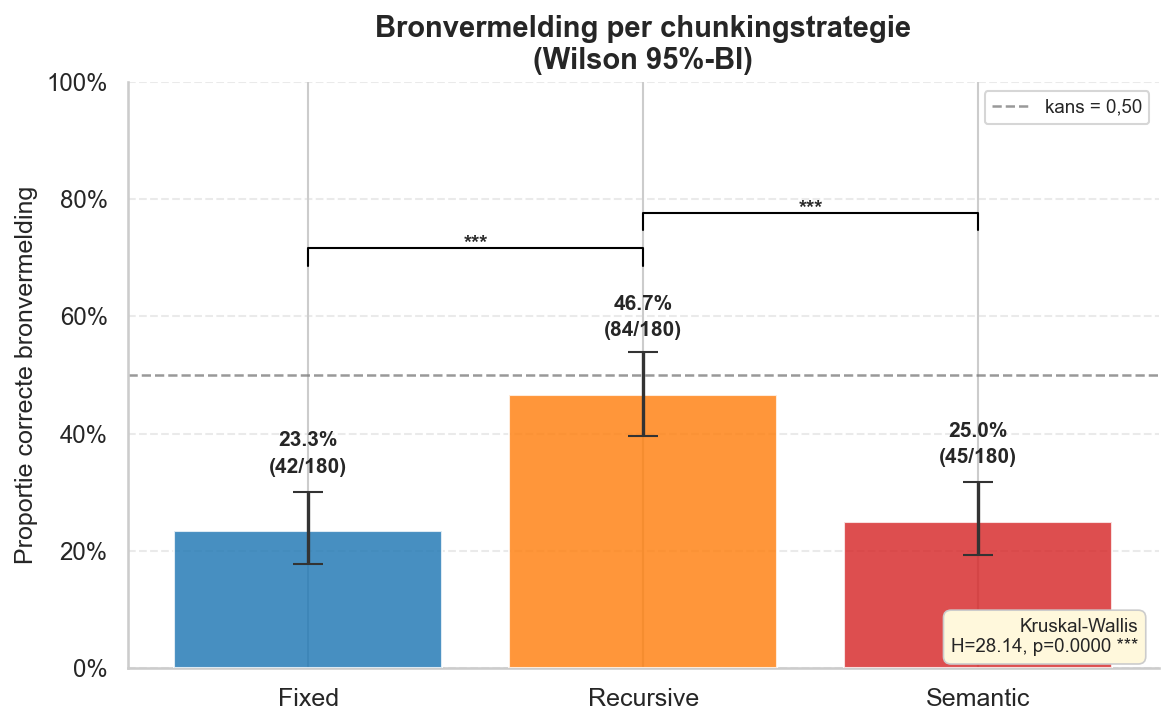
\includegraphics[width=0.80\textwidth]{../graphics/chunker_source_attribution.png}
  \caption[Proportie correcte bronvermelding per chunkingstrategie (Wilson 95\,\%-BI)]{Proportie correcte bronvermelding per chunkingstrategie (Wilson 95\,\%-BI). De \texttt{RecursiveCharacterSplitter} scoort significant hoger dan de overige twee strategieën. De stippellijn geeft de kansdrempel van $50\,\%$ aan.\footnotemark}
  \label{fig:chunker_source_attribution}
\end{figure}
\footnotetext{Post-hoc Dunn/Holm: Fixed vs.\ Recursive $p < 0{,}001^{***}$; Recursive vs.\ Semantic $p < 0{,}001^{***}$; Fixed vs.\ Semantic $p = 0{,}734$\,ns.}

De \texttt{RecursiveCharacterSplitter} scoort beduidend het hoogst ($46{,}7\%$; $84/180$ vragen), terwijl \texttt{Fixed} ($23{,}3\%$; $42/180$) en \texttt{Semantic} ($25{,}0\%$; $45/180$) vergelijkbaar en significant lager presteren. Enkel de \texttt{RecursiveCharacterSplitter} onderscheidt zich statistisch van de anderen (beide paren $p_{\text{holm}} < 0{,}001$); het verschil tussen \texttt{Fixed} en \texttt{Semantic} is verwaarloosbaar ($p_{\text{holm}} = 0{,}734$). Een binomiale proportietoets bevestigt dat de SA-score van \texttt{Recursive} ($46{,}7\%$, $\text{CI} = [39{,}5\%, 53{,}9\%]$) niet significant verschilt van de kansdrempel van $50\,\%$ ($p = 0{,}412$), terwijl \texttt{Fixed} en \texttt{Semantic} significant onder die drempel blijven ($p < 0{,}001$).

Dit patroon is causaal te verklaren door de structuurbehoudende werking van het recursieve algoritme. De \texttt{RecursiveCharacterSplitter} splitst op hiërarchische scheidingstekens (\texttt{\textbackslash n\textbackslash n}, \texttt{\textbackslash n}, punt-spatie), waardoor chunksegmenten doorgaans samenvallen met logische alinea- en sectiescheidingen in de originele PDF. Tegelijkertijd genereert de \texttt{RecursiveCharacterSplitter} significant grotere contextuele blokken dan de andere strategieën ($H = 154{,}77$, $p < 0{,}001$): gemiddeld $8.798$ prompt-tokens versus $7.484$ voor \texttt{Fixed} en $6.603$ voor \texttt{Semantic}. Door de grotere chunk-omvang blijven paginagrensmarkeerders en documenttitels integraal in het desbetreffende chunk aanwezig, wat het voor het LLM eenvoudiger maakt een valide bronverwijzing op te bouwen. De \texttt{FixedSizeTokenSplitter} kapt op vaste tokengrenzen die niet noodzakelijk samenvallen met paginagrenzen, waardoor citatie-metadata soms wordt doorgesneden. De \texttt{SemanticEmbeddingChunker} groepeert op basis van semantische coherentie, waardoor inhoud van verschillende pagina's in één chunk kan worden samengevat, wat de koppeling aan een exacte bronpagina minder evident maakt.

De causale kern van dit patroon is direct te koppelen aan de paginamarkeringslogica in de indexeringspipeline. De \texttt{DocumentCleaner} injecteert voor elke alinea van het samengebundelde document een markeerder in de vorm \texttt{<<<PAGE X>>>}; na het chunken extraheert de \texttt{ChunkMetaCleaner} uitsluitend de \textit{eerste} marker die in een chunk voorkomt en koppelt die als \texttt{page}-metadata aan het fragment (Secties~\ref{subsec:documentcleaner}--\ref{subsec:chunkmetacleaner}). Een chunkingalgoritme dat zo'n markeerder opsplitst, doet het resulterende fragment zijn paginanummer-ankerpunt verliezen.

De scheidingsteken-hiërarchie van de \texttt{RecursiveCharacterSplitter} — \texttt{["\textbackslash n\textbackslash n", "\textbackslash n", ". ", " ", ""]} — zorgt ervoor dat de splitsing bij voorkeur valt op alinea-grenzen (Sectie~\ref{subsec:recursive-chunker}): precies de posities waar de \texttt{DocumentCleaner} zijn paginamarkeerders heeft ingevoegd. De markeerder belandt hierdoor structureel aan het begin van een chunk, zodat de \texttt{ChunkMetaCleaner} de correcte paginawaarde kan extraheren. De \texttt{FixedSizeTokenSplitter} gebruikt uitsluitend \texttt{[" ", ""]} — woordgrenzen, nooit regelovergangen (Sectie~\ref{subsec:fixed-chunker}). Wanneer de tokengrens midden in een alineaovergang valt, wordt de paginamarkeerder losgerukt uit zijn context en gaat de paginawaarde verloren. Dit concrete verschil in scheidingsteken-architectuur — en niet een abstracte voorkeur voor structuurbehoud — is de onderliggende oorzaak van de statistisch significante SA-superioriteit van de \texttt{RecursiveCharacterSplitter}.

Een bijkomende observatie die de SA-scores voor Word-documenten beïnvloedt, is een systematische paginanummer-offset specifiek aan \texttt{.docx}-bestanden. Unstructured telt kopteksten en inhoudsopgaven als afzonderlijke paginaoppervlakken, waardoor de intern toegekende paginanummers bij \texttt{.docx}-bestanden consequent twee à drie pagina's hoger liggen dan de visuele paginanummering van het originele bestand. Dit veroorzaakt een structurele onderschatting van de SA-scores voor Word-documenten, aangezien de programmatische SA-controle de gerapporteerde paginanummers vergelijkt met de handmatig geannoteerde paginanummers in de golden dataset (Sectie~\ref{sec:golden-dataset-structuur}).

\subsection{Embeddingmodel}
\label{subsec:embedding-prestaties}

Het embeddingmodel is topologisch verantwoordelijk voor de wiskundige transformatie van tekstuele \gls{esg}-data naar continu verdeelde vectoren in een meerdimensionale vectorruimte. De structuur en semantische resolutie van deze vectorruimte bepalen de accuraatheid van de \textit{dense retrieval}-fase. De cross-component analyse identificeert het embeddingmodel als de primaire driver voor \textit{Context Recall}, \textit{Context Precision} en \textit{Answer Relevancy}, met een secundair effect op \textit{Source Attribution}.

\subsubsection{Context Recall}

De \textit{Context Recall} meet de mate waarin de pipeline erin slaagt om alle noodzakelijke, relevante informatie uit het \gls{esg}-brondocument boven water te halen. Het embeddingmodel is de primaire driver ($H = 7{,}54$, $p = 0{,}023$). Tabel~\ref{tab:stats-embedder-recall} documenteert de paarsgewijze Dunn-contrasten.

\begin{table}[!htb]
\centering
\begin{tabularx}{\textwidth}{@{}Xccc@{}}
\toprule
\textbf{Contrast / Statistische Indicator} & \textbf{Statistiek} & \textbf{$p$-waarde} & \textbf{Sign.} \\ \midrule
Kruskal-Wallis ($H$-test)                         & $H = 7{,}54$ & $= 0{,}023$ & * \\ \\[0.5em]
\texttt{E5-large} vs. \texttt{Snowflake}          & $z = 2{,}73$ & $p_{\text{holm}} = 0{,}019$ & * \\
\texttt{bge-m3} vs. \texttt{Snowflake}            & $z = 1{,}62$ & $p_{\text{holm}} = 0{,}210$ & ns \\
\texttt{bge-m3} vs. \texttt{E5-large}             & $z = 1{,}11$ & $p_{\text{holm}} = 0{,}268$ & ns \\
\bottomrule
\end{tabularx}
\textit{Noot.} Significantiecodes: * $p < 0{,}05$; ns = niet significant ($p \geq 0{,}05$).
\caption[KW + Dunn-post-hoc: Embedder op Context Recall]{Kruskal-Wallis basistoets en post-hoc Dunn-contrasten met Holm-correctie voor de geïsoleerde embeddingmodellen op Context Recall.}
\label{tab:stats-embedder-recall}
\end{table}

\begin{figure}[!htb]
    \centering
    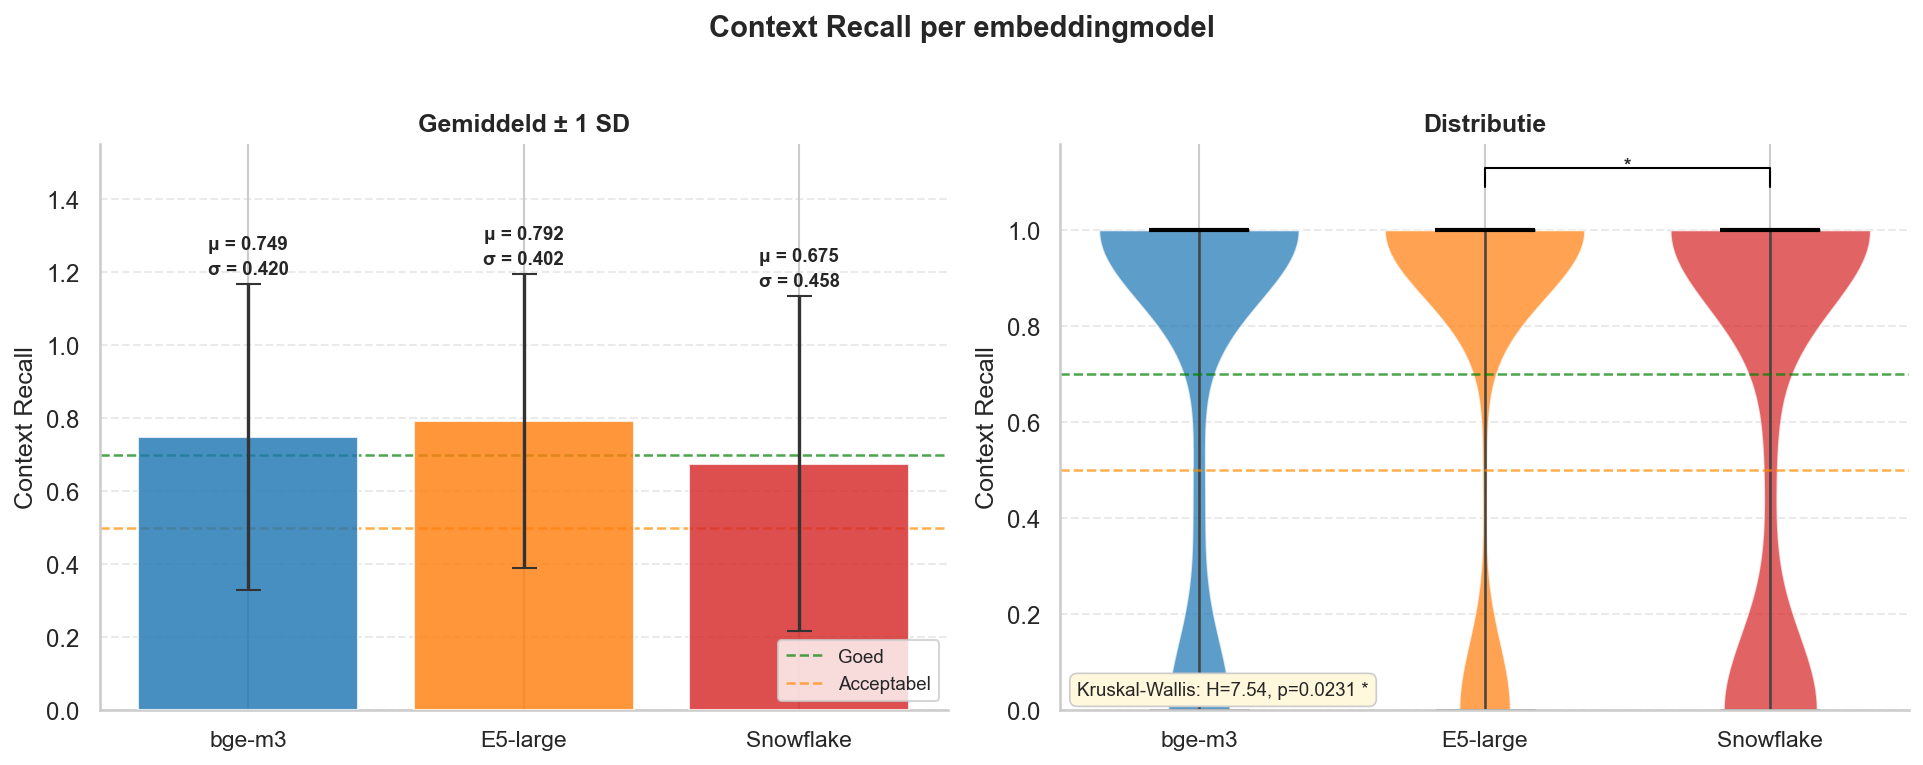
\includegraphics[width=\textwidth]{../graphics/embedder_02_context_recall.png}
    \caption[Context Recall per embeddingmodel]{Distributie van de Context Recall-scores per embeddingmodel (gemiddeld $\pm$ 1 SD en distributie). \texttt{E5-large} behaalt de hoogste gemiddelde recall ($\mu = 0{,}792$), significant beter dan \texttt{Snowflake} ($\mu = 0{,}675$). \texttt{bge-m3} ($\mu = 0{,}749$) neemt statistisch een middenpositie in.}
    \label{fig:embedder-recall}
\end{figure}

De post-hoc contrasten in Tabel~\ref{tab:stats-embedder-recall} onthullen een genuanceerd patroon dat afwijkt van intuïtieve verwachtingen. \texttt{multilingual-e5-large-instruct} behaalt de superieure gemiddelde recall van $\mu = 0{,}792$ en is statistisch significant beter dan de baseline \texttt{Snowflake} ($p_{\text{holm}} = 0{,}019$). Opmerkelijk is dat \texttt{BAAI/bge-m3} ($\mu = 0{,}749$) niet significant verschilt van \texttt{E5-large} ($p_{\text{holm}} = 0{,}268$) noch van \texttt{Snowflake} ($p_{\text{holm}} = 0{,}210$). \texttt{bge-m3} neemt bijgevolg een statistische middenpositie in. De hybride dense-sparse architectuur van \texttt{bge-m3}, die normaliter een retrievalvoordeel biedt, resulteert in dit \gls{esg}-corpus niet in een aantoonbaar hogere recall dan \texttt{E5-large}. Een plausibele verklaring is dat de grotere chunk-omvang in dit experiment de contextvensters van alle modellen ruimer maakt, waardoor de specifieke meerwaarde van de sparse retrieval-component van \texttt{bge-m3} minder uitgesproken wordt.

Bijzonder opmerkelijk is dat \texttt{E5-large} de hoogste recall behaalt ondanks een fundamentele architecturale beperking: de maximale inputlengte bedraagt slechts 512 tokens — expliciet gedocumenteerd in de longlist (Tabel~\ref{tab:embeddingmodels}). Chunks van tot 1.024 tokens worden tijdens de embedding-fase afgekapt op positie 512. Ruwweg 35\% van de chunk-inhoud (tokens 513–869) ontbreekt bijgevolg in de vectorindex. De chunk-overlap van 154 tokens dekt de grensgevallen gedeeltelijk af: de laatste 154 tokens van chunk $n$ (posities 870–1024) vallen wél in de eerste 512 tokens van chunk $n+1$ en worden daar alsnog geïndexeerd. Tokens 513–869 vormen echter een structurele blinde vlek zonder overlappende dekking.

Dat \texttt{E5-large} desondanks de sterkste recall realiseert, is verklaarbaar via drie samenlopende mechanismen. Ten eerste compenseert de instruction-tuning de beperkte contextcapaciteit. De \gls{esg}-gerichte instructieprefix (Tabel~\ref{tab:embedding-prefixes}) conditioneert de encoder op de retrieval-rol, waardoor de 512 tokens die wél worden verwerkt gerichter worden gecodeerd dan bij niet-instruction-tuned modellen met een ruimer contextvenster — een patroon dat~\textcite{WangEtAl2022} beschrijven voor de gehele E5-modelfamilie. Ten tweede zijn \gls{esg}-compliancedocumenten structureel \textit{front-loaded}: regelgevende clausules, kwantitatieve datapunten en ESRS-definities verschijnen doorgaans in de eerste zinnen van een passage, gevolgd door uitweidingen en voetnoten. De eerste 512 tokens bevatten hierdoor statistisch vaker het retrieval-relevante signaal. Ten derde treedt bij langere embeddings een \textit{verdunnings-effect} op: irrelevante tokens in een lange passage verzwakken het retrieval-signaal in de vectorrepresentatie. Een gefocust 512-tokenvenster kan voor topic-level matching effectiever zijn dan een volledig 1.024-tokenvenster met perifere context.

Dit resultaat valideert empirisch de methodologische keuze om de chunkgrootte niet specifiek voor \texttt{E5-large} te halveren (Sectie~\ref{sec:lokale-embedding}): een truncatie die op geaggregeerd niveau geen aantoonbare recall-penalisering veroorzaakt, rechtvaardigt geen afwijkende experimentele behandeling die de chunkgrootte als gecontroleerde variabele zou doorbreken.

De lagere retrievalkwaliteit van \texttt{Snowflake} is zorgwekkend voor een \gls{esg}-compliancecontext: wanneer relevante CSRD- en ESRS-clausules niet in de top-$k$ context worden opgenomen, raakt de downstream generatieve LLM fundamenteel 'uitgehongerd' qua feitenbasis, met een cascade-effect op zowel faithfulness als source attribution.

De zwakke retrievalprestaties van \texttt{Snowflake} zijn in het licht van de shortlist-selectie (Sectie~\ref{sec:shortlist-embedding}) opvallend: het model werd mede geselecteerd op basis van zijn uitstekende \gls{clef}-benchmarkscore voor Italiaanse retrieval ($\text{NDCG@10} = 0{,}541$), significant hoger dan \texttt{bge-m3} ($0{,}410$) en \texttt{E5-large} ($0{,}431$)~\autocite{YuEtAl2024}. De experimentele resultaten tonen het omgekeerde beeld. Twee implementatiefactoren verklaren deze discrepantie. Ten eerste is de \gls{mrl}-truncatie naar 256 dimensies (Sectie~\ref{sec:lokale-embedding}) een dimensionale reductie van factor vier ten opzichte van de volledige 1.024-dimensionale ruimte; de \gls{clef}-benchmark meet de volledige representatiecapaciteit, terwijl dit experiment de getrunceerde vectoren inzet. Ten tweede zijn de \gls{clef}-corpora opgebouwd uit journalistieke nieuwsteksten — een domein dat structureel verschilt van de technisch-juridische \gls{esg}-rapportages, ESRS-standaarden en kwantitatieve duurzaamheidstabellen in de dataset van Turtle Srl. Domeinverschuiving van een nieuws-benchmark naar een compliance-corpus verklaart waarom een hogere benchmarkscore voor algemene meertalige retrieval geen garantie biedt voor sectorspecifieke retrievalkwaliteit.

\subsubsection{Context Precision}

De \textit{Context Precision} evalueert de zuiverheid van het opgehaalde venster. Ook hier is de invloed van het embeddingmodel doorslaggevend ($H = 13{,}69$, $p = 0{,}001$). Tabel~\ref{tab:stats-embedder-precision} documenteert de statistisch significante contrasten.

\begin{table}[!htb]
\centering
\begin{tabularx}{\textwidth}{@{}Xccc@{}}
\toprule
\textbf{Contrast / Statistische Indicator} & \textbf{Statistiek} & \textbf{$p$-waarde} & \textbf{Sign.} \\ \midrule
Kruskal-Wallis ($H$-test)                         & $H = 13{,}69$ & $= 0{,}001$                 & ** \\ \nopagebreak
\texttt{E5-large} vs. \texttt{Snowflake}          & $z = 3{,}62$  & $p_{\text{holm}} < 0{,}001$ & *** \\
\texttt{bge-m3} vs. \texttt{Snowflake}            & $z = 2{,}29$  & $p_{\text{holm}} = 0{,}038$ & * \\
\texttt{bge-m3} vs. \texttt{E5-large}             & $z = 1{,}33$  & $p_{\text{holm}} = 0{,}192$ & ns \\
\bottomrule
\end{tabularx}
\textit{Noot.} Significantiecodes: *** $p < 0{,}001$; * $p < 0{,}05$; ns = niet significant ($p \geq 0{,}05$).
\caption[KW + Dunn-post-hoc: Embedder op Context Precision]{Kruskal-Wallis basistoets en post-hoc Dunn-contrasten met Holm-correctie voor de geïsoleerde embeddingmodellen op Context Precision.}
\label{tab:stats-embedder-precision}
\end{table}

\begin{figure}[!htb]
    \centering
    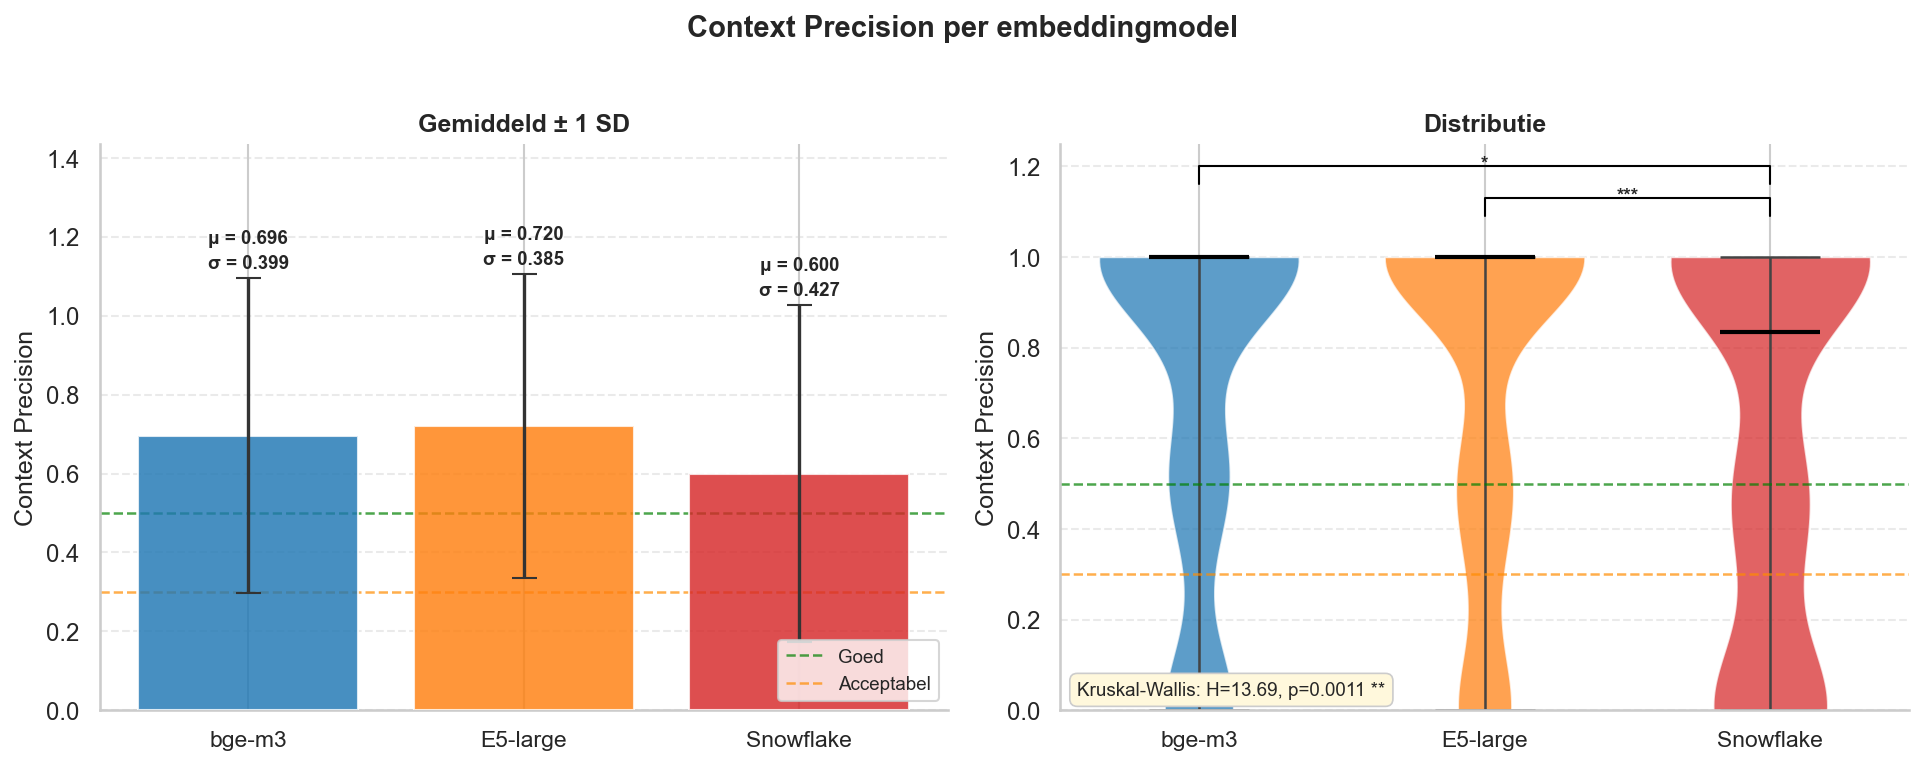
\includegraphics[width=\textwidth]{../graphics/embedder_03_context_precision.png}
    \caption[Context Precision per embeddingmodel]{Distributie van de Context Precision-scores per embeddingmodel. \texttt{E5-large} ($\mu = 0{,}720$) en \texttt{bge-m3} ($\mu = 0{,}696$) zijn statistisch equivalent aan elkaar en beide significant beter dan \texttt{Snowflake} ($\mu = 0{,}600$).}
    \label{fig:embedder-precision}
\end{figure}

Voor \textit{Context Precision} treedt een duidelijke tweedeling op. \texttt{E5-large} ($\mu = 0{,}720$) en \texttt{bge-m3} ($\mu = 0{,}696$) vertonen een statistisch equivalent prestatieprofiel ($p_{\text{holm}} = 0{,}192$), en beide laten de baseline \texttt{Snowflake} ($\mu = 0{,}600$) significant achter zich ($p_{\text{holm}} < 0{,}001$ respectievelijk $p_{\text{holm}} = 0{,}038$). De distributie van \texttt{Snowflake} in Figuur~\ref{fig:embedder-precision} toont een duidelijk bredere spreiding met een lagere mediaan. Dit model slaagt er onvoldoende in om de meest kritieke chunks consistent in de top van de ranking te plaatsen, waardoor werkelijk relevante context dieper in de prompt wegzakt. Dit verhoogt het risico op foutieve interpretaties bij de generatiefase en tast de faithfulness stroomafwaarts aan.

\subsubsection{Answer Relevancy}

Een nieuwe empirische bevinding van dit experiment is dat het embeddingmodel de primaire driver is voor \textit{Answer Relevancy} ($H = 13{,}82$, $p = 0{,}001$). Tabel~\ref{tab:stats-embedder-relevancy} toont de paarsgewijze contrasten.

\begin{table}[!htb]
\centering
\begin{tabularx}{\textwidth}{@{}Xccc@{}}
\toprule
\textbf{Contrast / Statistische Indicator} & \textbf{Statistiek} & \textbf{$p$-waarde} & \textbf{Sign.} \\ \midrule
Kruskal-Wallis ($H$-test)                  & $H = 13{,}82$ & $= 0{,}001$                 & *** \\ \nopagebreak
\texttt{bge-m3} vs. \texttt{Snowflake}    & $z = 3{,}70$  & $p_{\text{holm}} < 0{,}001$ & *** \\
\texttt{E5-large} vs. \texttt{Snowflake}  & $z = 2{,}18$  & $p_{\text{holm}} = 0{,}058$ & ns  \\
\texttt{bge-m3} vs. \texttt{E5-large}     & $z = 1{,}52$  & $p_{\text{holm}} = 0{,}129$ & ns  \\
\bottomrule
\end{tabularx}
\textit{Noot.} Significantiecodes: *** $p < 0{,}001$; ns = niet significant ($p \geq 0{,}05$).
\caption[KW + Dunn-post-hoc: Embedder op Answer Relevancy]{Kruskal-Wallis basistoets en post-hoc Dunn-contrasten met Holm-correctie voor de geïsoleerde embeddingmodellen op Answer Relevancy.}
\label{tab:stats-embedder-relevancy}
\end{table}

\texttt{BAAI/bge-m3} behaalt de hoogste gemiddelde antwoordrelevantie ($\mu = 0{,}679$) en is statistisch significant beter dan \texttt{Snowflake} ($\mu = 0{,}546$, $p_{\text{holm}} < 0{,}001$). Het verschil met \texttt{E5-large} ($\mu = 0{,}635$) is niet statistisch significant ($p_{\text{holm}} = 0{,}129$). Dit resultaat legt een inverse prestatiehiërarchie bloot ten opzichte van de recall-resultaten: waar \texttt{E5-large} de beste \textit{Context Recall} behaalt, presteert \texttt{bge-m3} het best op \textit{Answer Relevancy}. De verklaring ligt in de aard van de twee metrics: context recall beloont het ophalen van een grote hoeveelheid relevante informatie, terwijl answer relevancy beloont dat de geselecteerde context direct aansluit bij de vraagintentie. De multi-vector architectuur van \texttt{bge-m3} — die zowel dense als sparse representaties combineert — blinkt uit in het identificeren van de meest on-topic passages, wat zich vertaalt in een hogere focuskwaliteit van de gegenereerde antwoorden.

\begin{figure}[!htb]
    \centering
    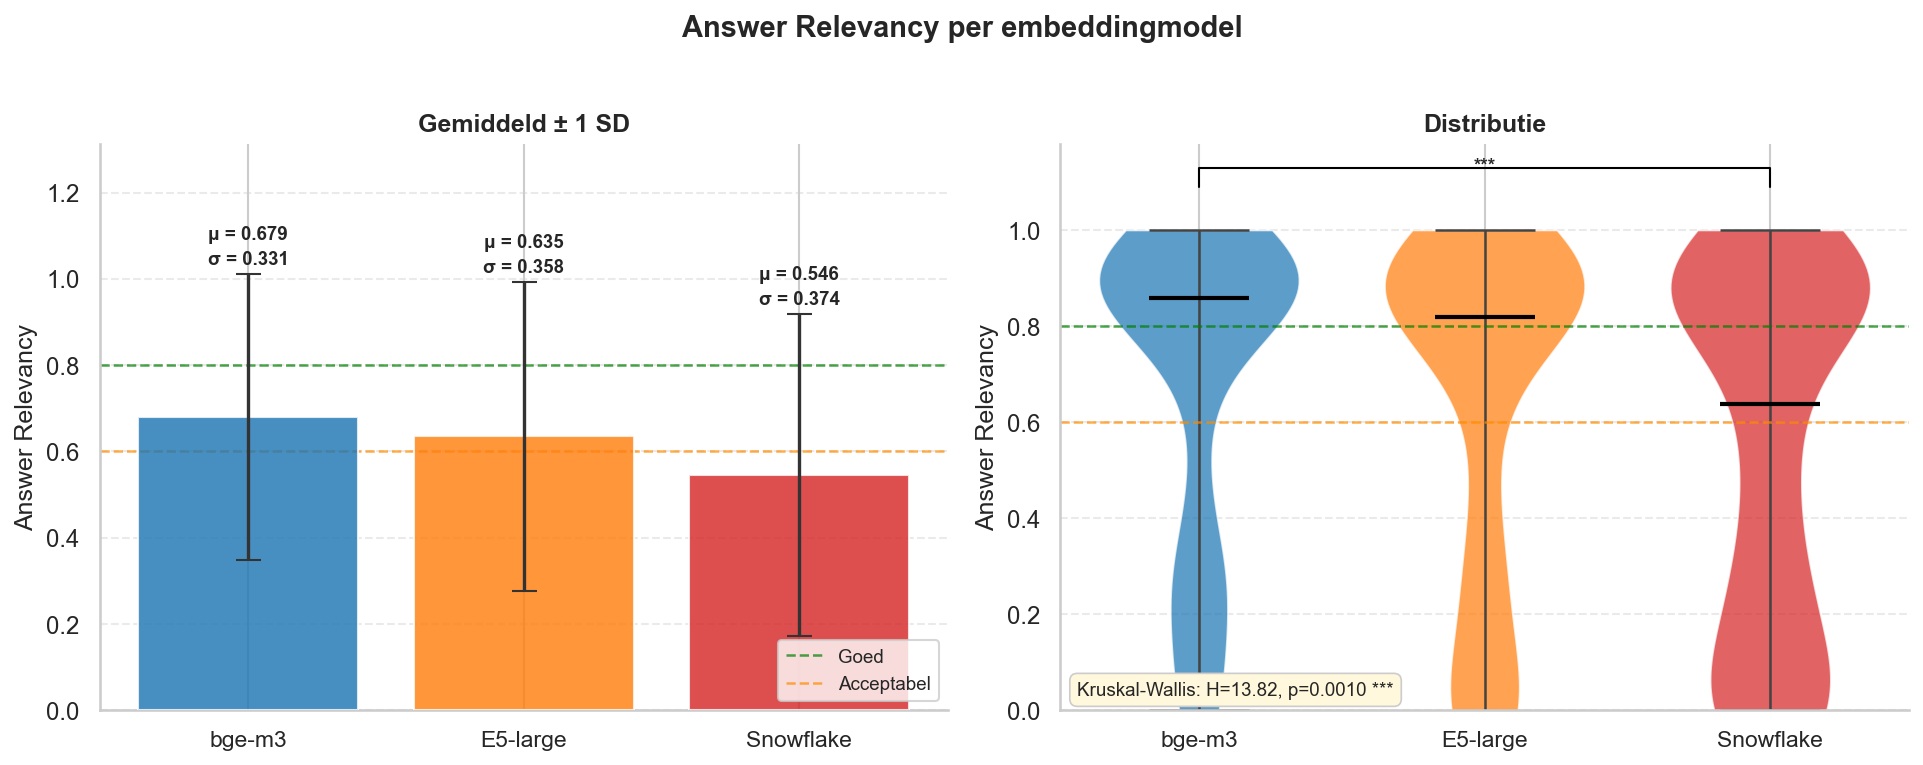
\includegraphics[width=\textwidth]{../graphics/embedder_04_answer_relevancy.png}
    \caption[Answer Relevancy per embeddingmodel]{Distributie van de Answer Relevancy-scores
    per embeddingmodel. \texttt{bge-m3} ($\mu = 0{,}679$) is significant beter dan
    \texttt{Snowflake} ($\mu = 0{,}546$; $p_{\text{holm}} < 0{,}001$). Het verschil met
    \texttt{E5-large} ($\mu = 0{,}635$) is niet statistisch significant
    ($p_{\text{holm}} = 0{,}129$).}
    \label{fig:embedder-relevancy}
\end{figure}

\subsubsection{Source Attribution}

De \textit{Source Attribution} vertoont ook een significant embedder-effect ($H = 8{,}97$, $p = 0{,}011$), maar met een verrassende rangorde. \texttt{Snowflake} behaalt de hoogste gemiddelde SA-score ($\mu = 0{,}372$), gevolgd door \texttt{E5-large} ($\mu = 0{,}344$). \texttt{BAAI/bge-m3} behaalt de laagste SA-score ($\mu = 0{,}233$) en verschilt significant van zowel \texttt{E5-large} ($p_{\text{holm}} = 0{,}047$) als \texttt{Snowflake} ($p_{\text{holm}} = 0{,}014$). \texttt{E5-large} en \texttt{Snowflake} zijn niet significant van elkaar verschillend ($p_{\text{holm}} = 0{,}571$).

Dit inverse patroon — \texttt{bge-m3} presteert het best op retrieval maar het slechtst op bronvermelding — is te verklaren door de wisselwerking tussen de embedding-vectorisatie en de chunkmorfologie. De hybride dense-sparse architectuur van \texttt{bge-m3} selecteert bij voorkeur chunks die semantisch het meest representatief zijn voor de vraag, ongeacht hun fysieke positie in het originele document. Wanneer deze semantisch geselecteerde chunks metadata-arm zijn (bijvoorbeeld door het ontbreken van expliciete paginanummers), raakt het \gls{llm} zijn ankerpunt voor bronattributie kwijt. \texttt{E5-large} en \texttt{Snowflake} voeren daarentegen een conservatievere retrieval uit die sterker leunt op de documentstructuur, wat resulteert in chunks waarbij de paginamarkeringen vaker intact blijven.

Een preciezere causale verklaring voor dit inverspatroon ligt in de asymmetrische retrieval-architectuur. Voor \texttt{bge-m3} gebruikt de querypipeline de \texttt{QdrantHybridRetriever}, die dense en sparse zoekresultaten combineert via \gls{rrf} (Sectie~\ref{sec:query-pipeline}). De sparse lexicale gewichten van \texttt{bge-m3} kennen hoge retrieval-scores toe aan chunks die \gls{esg}-specifieke termen bevatten — kwantitatieve tabelrijen met ESRS-trefwoorden, percentages en emissiewaarden. Dergelijke tabelchunks liggen doorgaans centraal in een pagina zonder een \texttt{<<<PAGE X>>>}-markeerder aan het begin, waardoor de \texttt{ChunkMetaCleaner} geen paginametadata kan koppelen (Sectie~\ref{subsec:chunkmetacleaner}). \texttt{E5-large} en \texttt{Snowflake} gebruiken de \texttt{QdrantEmbeddingRetriever} (dense-only), die gradueler rankt op globale semantische gelijkenis en daardoor vaker chunks selecteert die aansluiten bij het begin van een alinea — precies de posities waar de paginamarkeerders staan ingevoegd.

\begin{table}[!htb]
\centering
\begin{tabularx}{\textwidth}{@{}Xccc@{}}
\toprule
\textbf{Contrast / Statistische Indicator} & \textbf{Statistiek} & \textbf{$p$-waarde} & \textbf{Sign.} \\ \midrule
Kruskal-Wallis ($H$-test)                  & $H = 8{,}97$ & $= 0{,}011$                 & *  \\ \nopagebreak
\texttt{bge-m3} vs. \texttt{E5-large}     & $z = 2{,}26$ & $p_{\text{holm}} = 0{,}047$ & *  \\
\texttt{bge-m3} vs. \texttt{Snowflake}    & $z = 2{,}83$ & $p_{\text{holm}} = 0{,}014$ & *  \\
\texttt{E5-large} vs. \texttt{Snowflake}  & $z = 0{,}57$ & $p_{\text{holm}} = 0{,}571$ & ns \\
\bottomrule
\end{tabularx}
\textit{Noot.} Significantiecodes: * $p < 0{,}05$; ns = niet significant ($p \geq 0{,}05$).
\caption[KW + Dunn-post-hoc: Embedder op Source Attribution]{Kruskal-Wallis basistoets en post-hoc Dunn-contrasten met Holm-correctie voor de geïsoleerde embeddingmodellen op Source Attribution. \texttt{bge-m3} verschilt significant van beide andere embedders; \texttt{E5-large} en \texttt{Snowflake} zijn statistisch equivalent.}
\label{tab:stats-embedder-sa}
\end{table}

\begin{figure}[!htb]
    \centering
    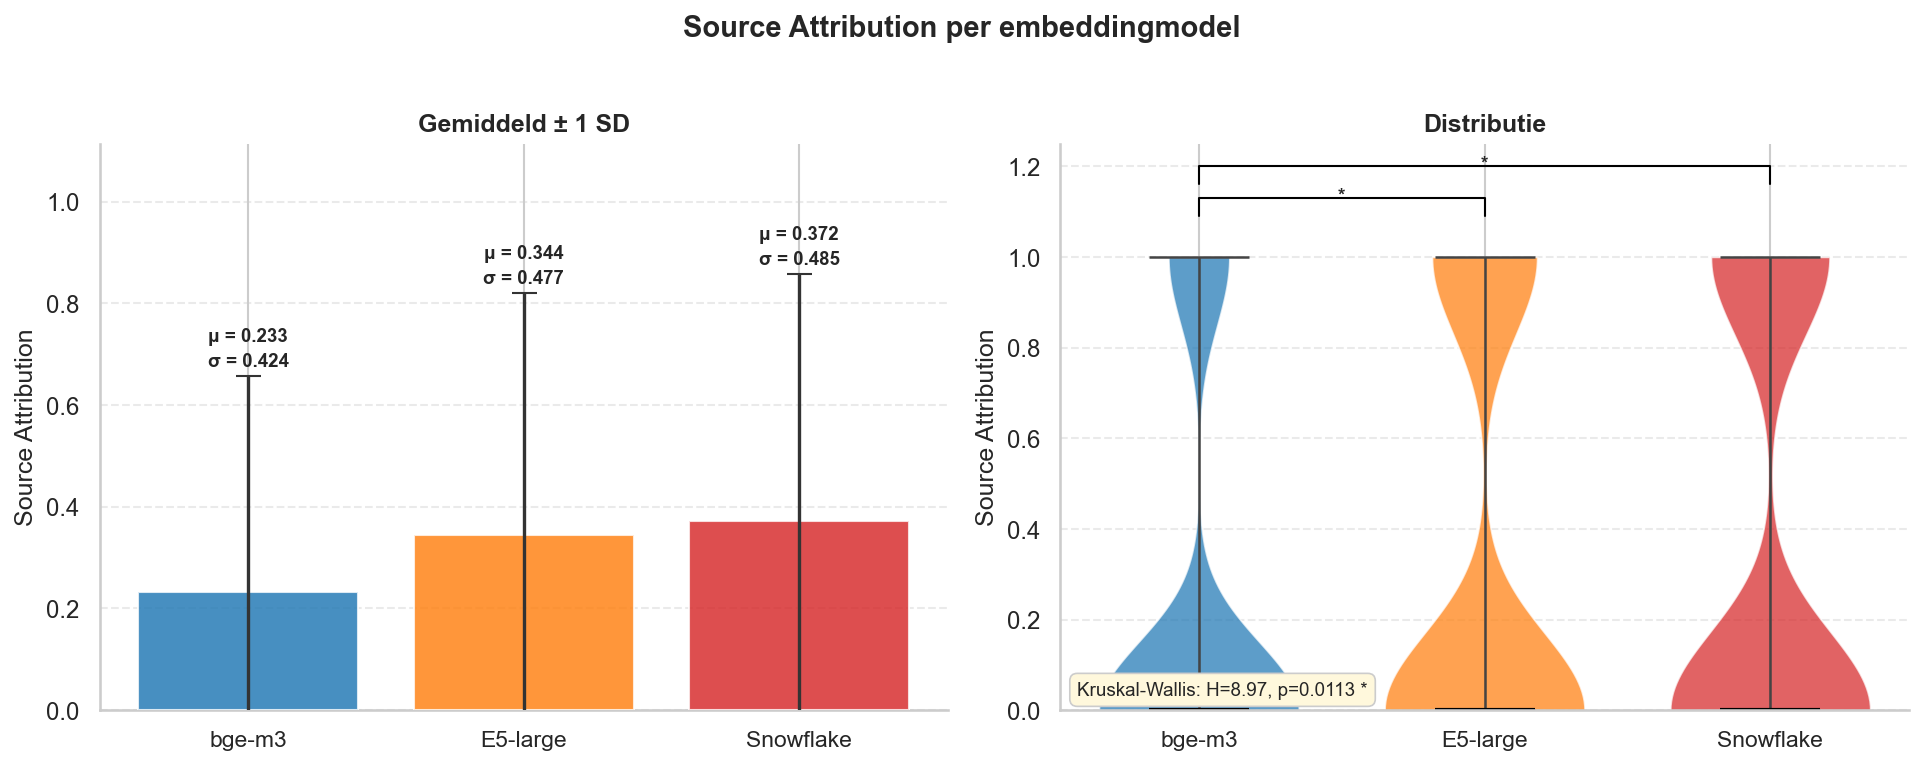
\includegraphics[width=\textwidth]{../graphics/embedder_05_source_attribution.png}
    \caption[Source Attribution per embeddingmodel]{Distributie van de Source Attribution-scores per embeddingmodel. \texttt{Snowflake} ($\mu = 0{,}372$) en \texttt{E5-large} ($\mu = 0{,}344$) zijn statistisch equivalent ($p_{\text{holm}} = 0{,}571$). \texttt{bge-m3} behaalt significant de laagste SA ($\mu = 0{,}233$; $p_{\text{holm}} \leq 0{,}047$ t.o.v.\ beide anderen) — een inverspatroon ten opzichte van de AR-resultaten (Figuur~\ref{fig:embedder-relevancy}).}
    \label{fig:embedder-sa}
\end{figure}

\subsection{Large Language Model}
\label{subsec:llm-prestaties}

De generatieve component — het Large Language Model — transformeert de opgehaalde \gls{esg}-context naar een coherent, feitelijk onderbouwd auditrapport. Conform de cross-component variantie-analyse (Tabel~\ref{tab:kw_cross_component}) blijkt het LLM in de huidige benchmark-configuratie \textit{geen} statistisch significante primaire driver te zijn voor \textit{Faithfulness} noch voor \textit{Answer Relevancy}.

De afwezigheid van een significant LLM-effect is niet een teken van gelijkwaardigheid, maar een direct gevolg van de gewijzigde chunkingparameters in dit experiment. Door de hogere tokenlimieten per chunk ($\max = 1024$ voor \texttt{Fixed}/\texttt{Recursive}) ontvangen alle drie de LLM's een substantieel rijkere contextbasis. Wanneer de context compleet genoeg is voor alle modellen, neemt de variatie in faithfulness tussen configuraties af en worden componenteffecten statistisch niet meer onderscheidbaar.

\subsubsection{Richting van de effecten op Faithfulness en Answer Relevancy}

Hoewel geen van de drie LLM's een statistisch significant verschil vertoont op \textit{Faithfulness} ($H = 5{,}78$, $p = 0{,}056$) noch op \textit{Answer Relevancy} ($H = 5{,}00$, $p = 0{,}082$), zijn de richtingspatronen instructief. Figuur~\ref{fig:llm-faithfulness} en Figuur~\ref{fig:llm-relevancy} tonen de distributies per LLM.

\begin{figure}[!htb]
    \centering
    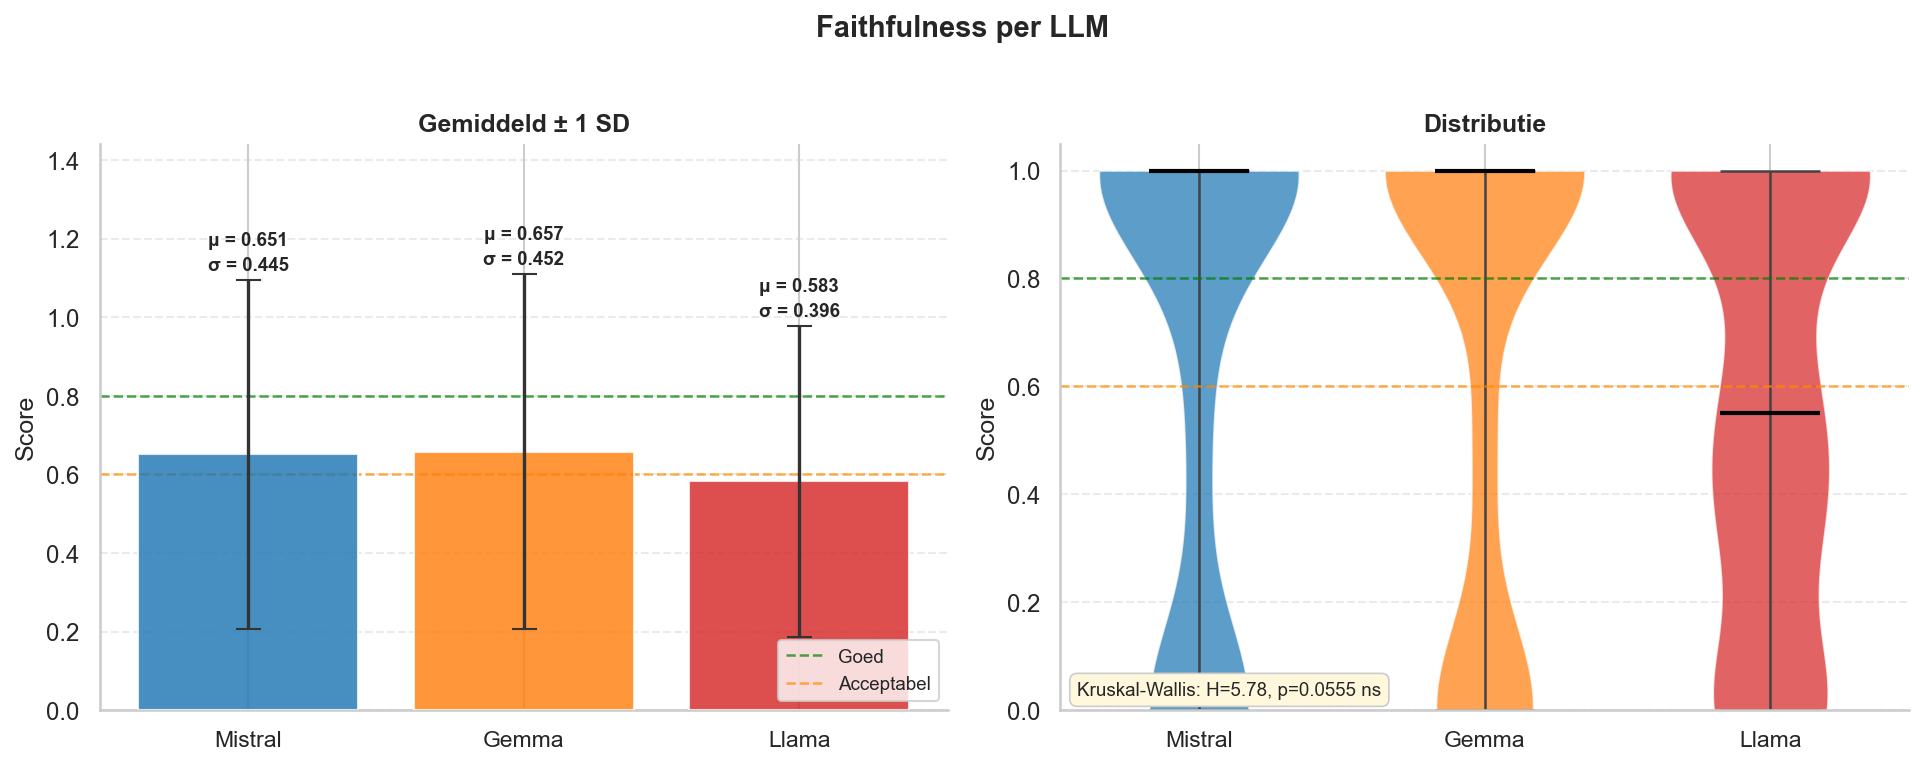
\includegraphics[width=\textwidth]{../graphics/llm_04_faithfulness.png}
    \caption[Faithfulness per LLM]{Distributie van de Faithfulness-scores per Large Language Model. De verschillen tussen \texttt{Mistral} ($\mu = 0{,}651$), \texttt{Gemma} ($\mu = 0{,}657$) en \texttt{Llama} ($\mu = 0{,}583$) zijn statistisch niet significant ($H = 5{,}78$, $p = 0{,}056$). \texttt{Llama} vertoont numeriek de laagste mediaan en de bredere spreiding, wat een tendens naar lagere feitelijke gronding suggereert zonder dat dit op groepsniveau statistisch bevestigd wordt.}
    \label{fig:llm-faithfulness}
\end{figure}

\begin{figure}[!htb]
    \centering
    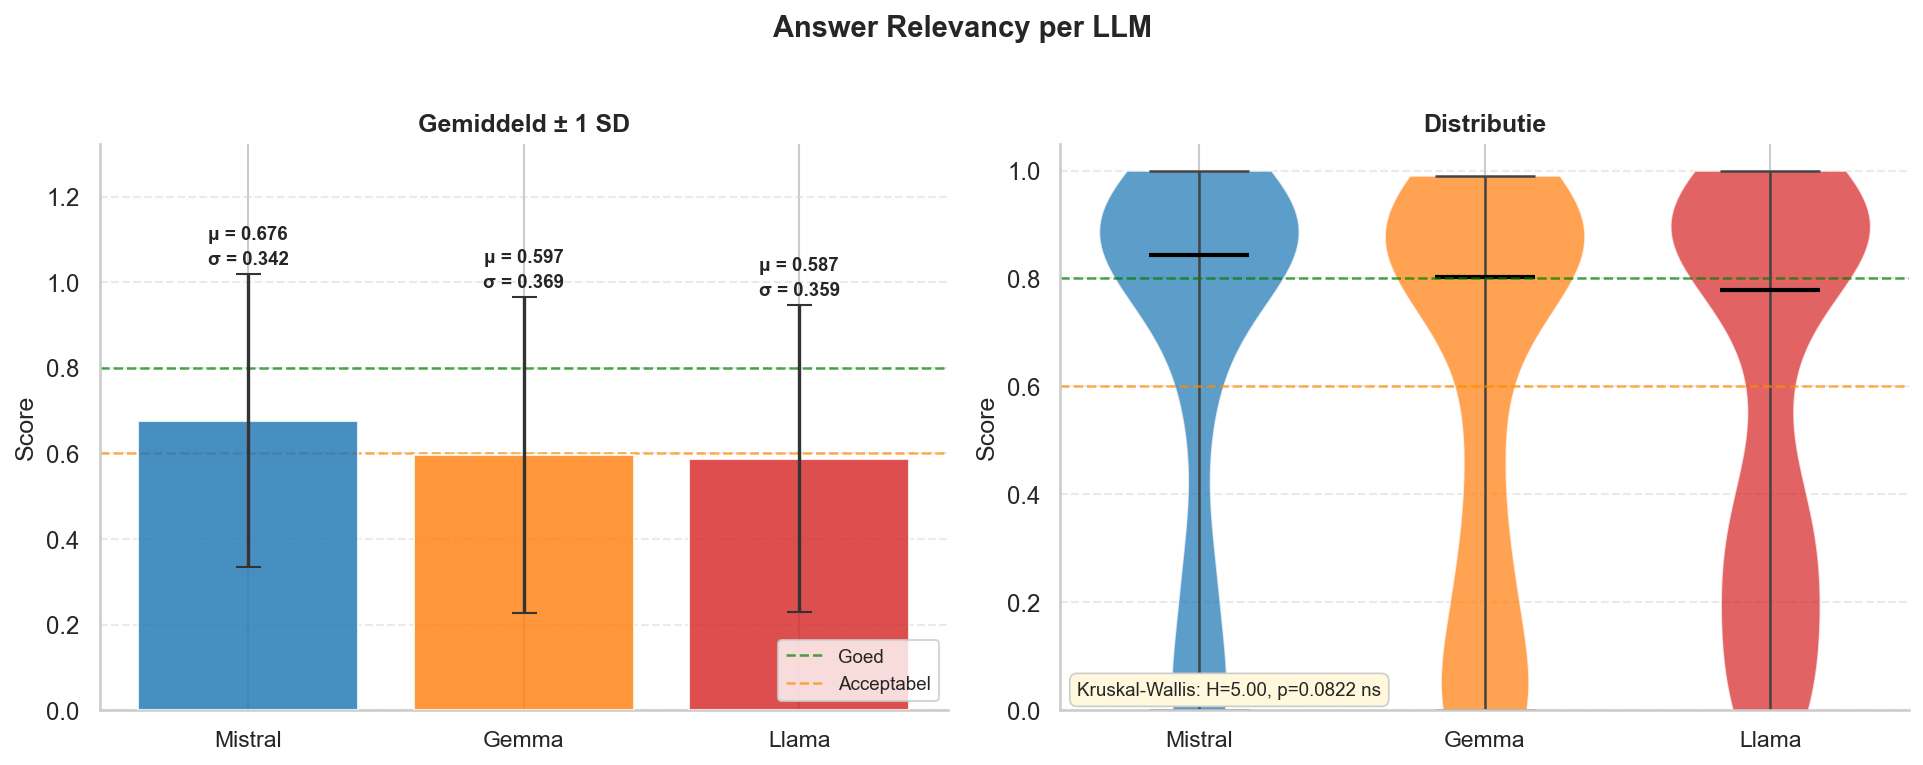
\includegraphics[width=\textwidth]{../graphics/llm_05_answer_relevancy.png}
    \caption[Answer Relevancy per LLM]{Distributie van de Answer Relevancy-scores per Large Language Model. \texttt{Mistral} behaalt numeriek de hoogste gemiddelde antwoordrelevantie ($\mu = 0{,}676$), maar het globale Kruskal-Wallis-effect is niet statistisch significant ($H = 5{,}00$, $p = 0{,}082$). \texttt{Gemma} ($\mu = 0{,}597$) en \texttt{Llama} ($\mu = 0{,}587$) tonen vergelijkbare distributies.}
    \label{fig:llm-relevancy}
\end{figure}

\texttt{Llama-3.3-70B-Instruct} vertoont in beide distributies een bredere spreiding en een lager gemiddelde dan de twee kleinere modellen. De $p$-waarden van $0{,}056$ en $0{,}082$ bevinden zich in de statistische grijze zone: ze overschrijden de $\alpha = 0{,}05$-drempel maar wijzen op een effect dat bij grotere steekproeven of variëteitsrijkere vragensets naar significantie zou kunnen converteren. Een grotere modelomvang biedt dus geen garantie op betere feitelijke verankering of antwoordrelevantie; de structuur van de aangeboden context is daarvoor doorslaggevender dan de modelgrootte.

\subsubsection{De Mistral-weigeringsparadox en het effect op Source Attribution}
\label{subsec:mistral-paradox}

Een opmerkelijk kwaliteitspatroon treedt op wanneer \texttt{Mistral-Small-2603} wordt gekoppeld aan suboptimale upstream-componenten. Wanneer de retrievalfase een gefragmenteerde of incomplete context oplevert — typisch het geval bij \texttt{Snowflake} als embedder — reageert \texttt{Mistral-Small} consequent met een formele weigering: ``\textit{Ik kan deze vraag niet beantwoorden op basis van de verstrekte documenten}''. Dit weigeringsgedrag is feitelijk de correcte reactie op een defecte retrievalfase: het model weigert te hallucineren. Het heeft echter een directe impact op de \textit{Source Attribution}-score, die voor elk weigeringsantwoord automatisch $0$ bedraagt omdat er geen brondocument wordt geciteerd.

De specifieke implementatiecontext versterkt dit structurele effect. Het promptsjabloon verplicht alle \glspl{llm} tot uitvoer in geldig \gls{json}-formaat inclusief een expliciet bronvermeldingsveld (Sectie~\ref{subsec:prompt-template}). \texttt{Mistral-Small} produceert ook bij een weigering een syntactisch valide \gls{json}-object — conform zijn sterke instructieopvolgingscapaciteiten — maar met een afwezig of \texttt{null} bronvermeldingsveld. De programmatische SA-controle detecteert het ontbreken van bestandsnaam en paginanummer, en kent automatisch de score $0$ toe. \texttt{Gemma-3-27b-it} en \texttt{Llama-3.3-70B-Instruct} trachten ook bij onvolledige context een antwoord te formuleren: de metadata van de opgehaalde chunks — bestandsnaam en paginanummer — is expliciet zichtbaar in het promptsjabloon (Sectie~\ref{subsec:prompt-template}), waardoor deze modellen de broninformatie structureel kunnen overnemen uit de aangeleverde context, ook wanneer het inhoudelijke antwoord suboptimaal is. Dit architecturale verschil in weigeringsgedrag verklaart dus gedeeltelijk de SA-kloof tussen \texttt{Mistral} en de twee andere modellen.

\begin{figure}[!htb]
    \centering
    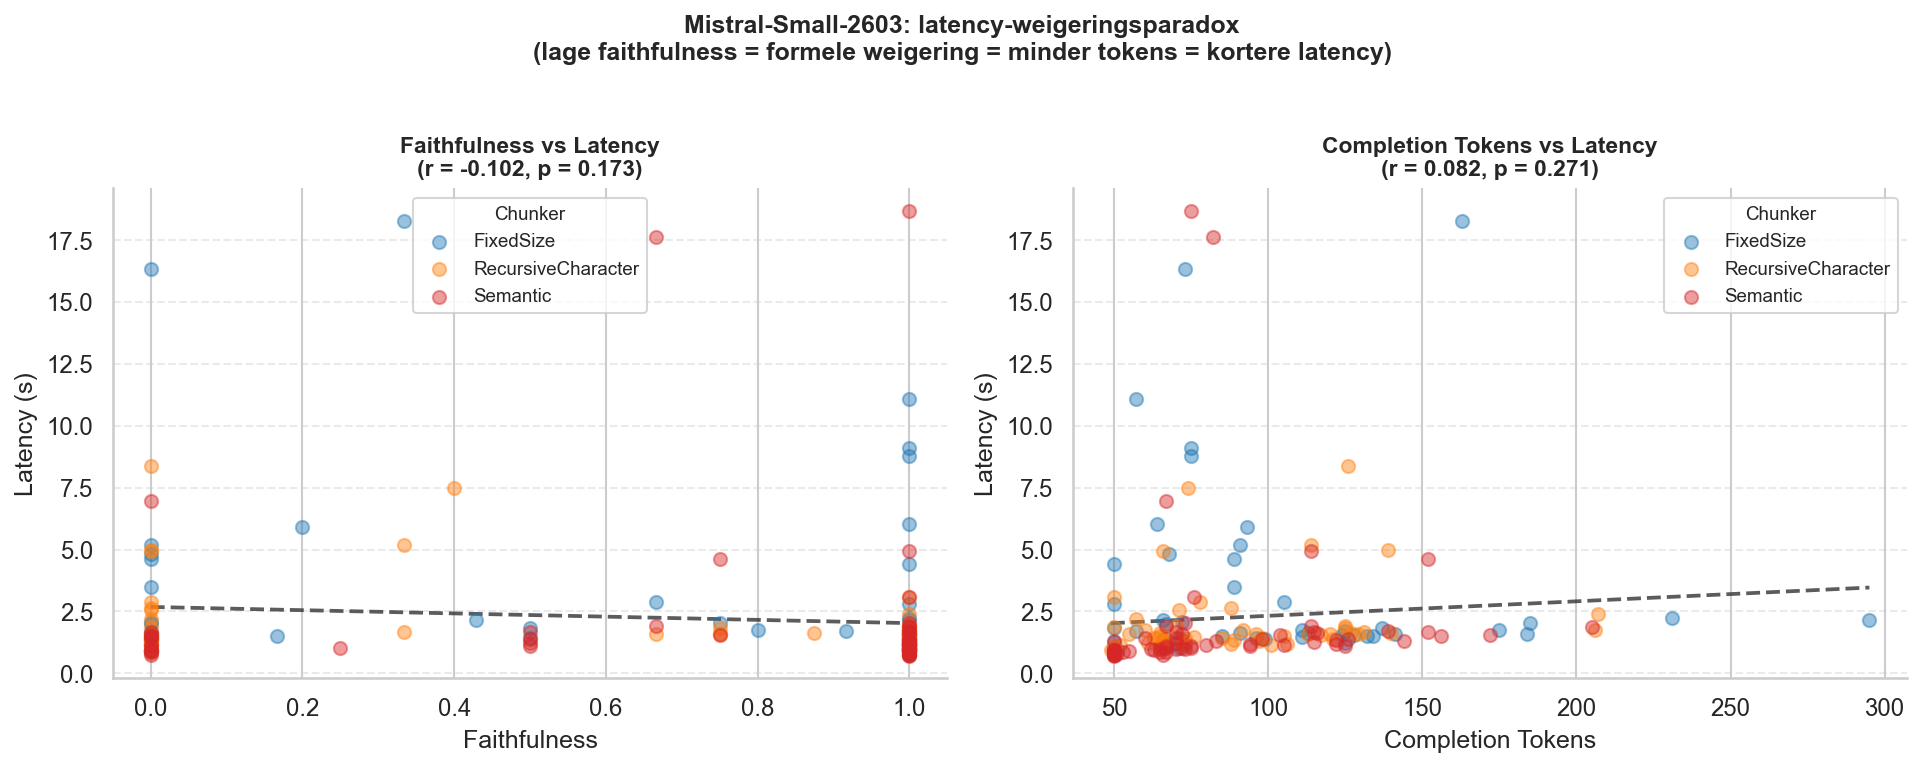
\includegraphics[width=\textwidth]{../graphics/latency_08_mistral_paradox.png}
    \caption[Weigeringsparadox bij Mistral-Small-2603]{De weigeringsparadox bij \texttt{Mistral-Small-2603}: een kortere verwerkingstijd correleert met het \texttt{Snowflake}-embeddingmodel (lagere retrievalkwaliteit), omdat het model bij ontoereikende context overgaat tot bondige weigeringsantwoorden. Dit toont aan dat een kortere responsduur bij Mistral een indicator is van retrieval-falen en een lagere Source Attribution, niet van efficiëntie.}
    \label{fig:mistral-paradox}
\end{figure}

Figuur~\ref{fig:mistral-paradox} maakt dit patroon zichtbaar. Configuraties met \texttt{Snowflake} produceren bij \texttt{Mistral} bondiger antwoorden, precies omdat weigeringen syntactisch minimaal zijn. Dit is geen operationele meerwaarde maar een kwaliteitsachteruitgang: de SA-score van \texttt{Mistral-Small} ($\mu = 0{,}278$) is lager dan die van \texttt{Gemma} ($\mu = 0{,}344$) en \texttt{Llama} ($\mu = 0{,}328$), wat deels verklaard wordt door dit weigeringsgedrag bij zwakke retrieval. \texttt{Gemma} en \texttt{Llama} trachten ook bij incomplete context een antwoord te formuleren, waardoor ze kansen op correcte bronvermelding behouden — zij het met het risico van hallucinaties. Het weigeringsgedrag van \texttt{Mistral} is audittechnisch integer maar drukt de SA-score structureel omlaag wanneer het embedder-chunker-paar ondermaats presteert. Dit onderstreept opnieuw dat de LLM pas optimaal kan presteren wanneer de upstream retrievalfase kwalitatief hoogwaardig is.

\section{Meervoudige variabele component-interactie}
\label{sec:meervoudige-interactie}

Waar de voorgaande secties de pipeline-parameters rigoureus isoleerden, dwingt de systeemdynamica van een RAG-pipeline tot een evaluatie van onderlinge component-interacties. De cross-component analyse toont dat de chunkingstrategie een statistisch significante, indirecte invloed uitoefent op de \textit{Context Precision} ($H = 6{,}98$, $p = 0{,}031$). Om de samengestelde dynamiek over de totale retrievalfase bloot te leggen, zijn de prestaties van alle unieke Chunker $\times$ Embedder-combinaties gerangschikt op gecombineerde retrievalkwaliteit — de gemiddelde score op zowel Context Recall als Context Precision. De finale ranking is gevisualiseerd in Figuur~\ref{fig:retriever-ranking}.

\begin{figure}[!htb]
    \centering
    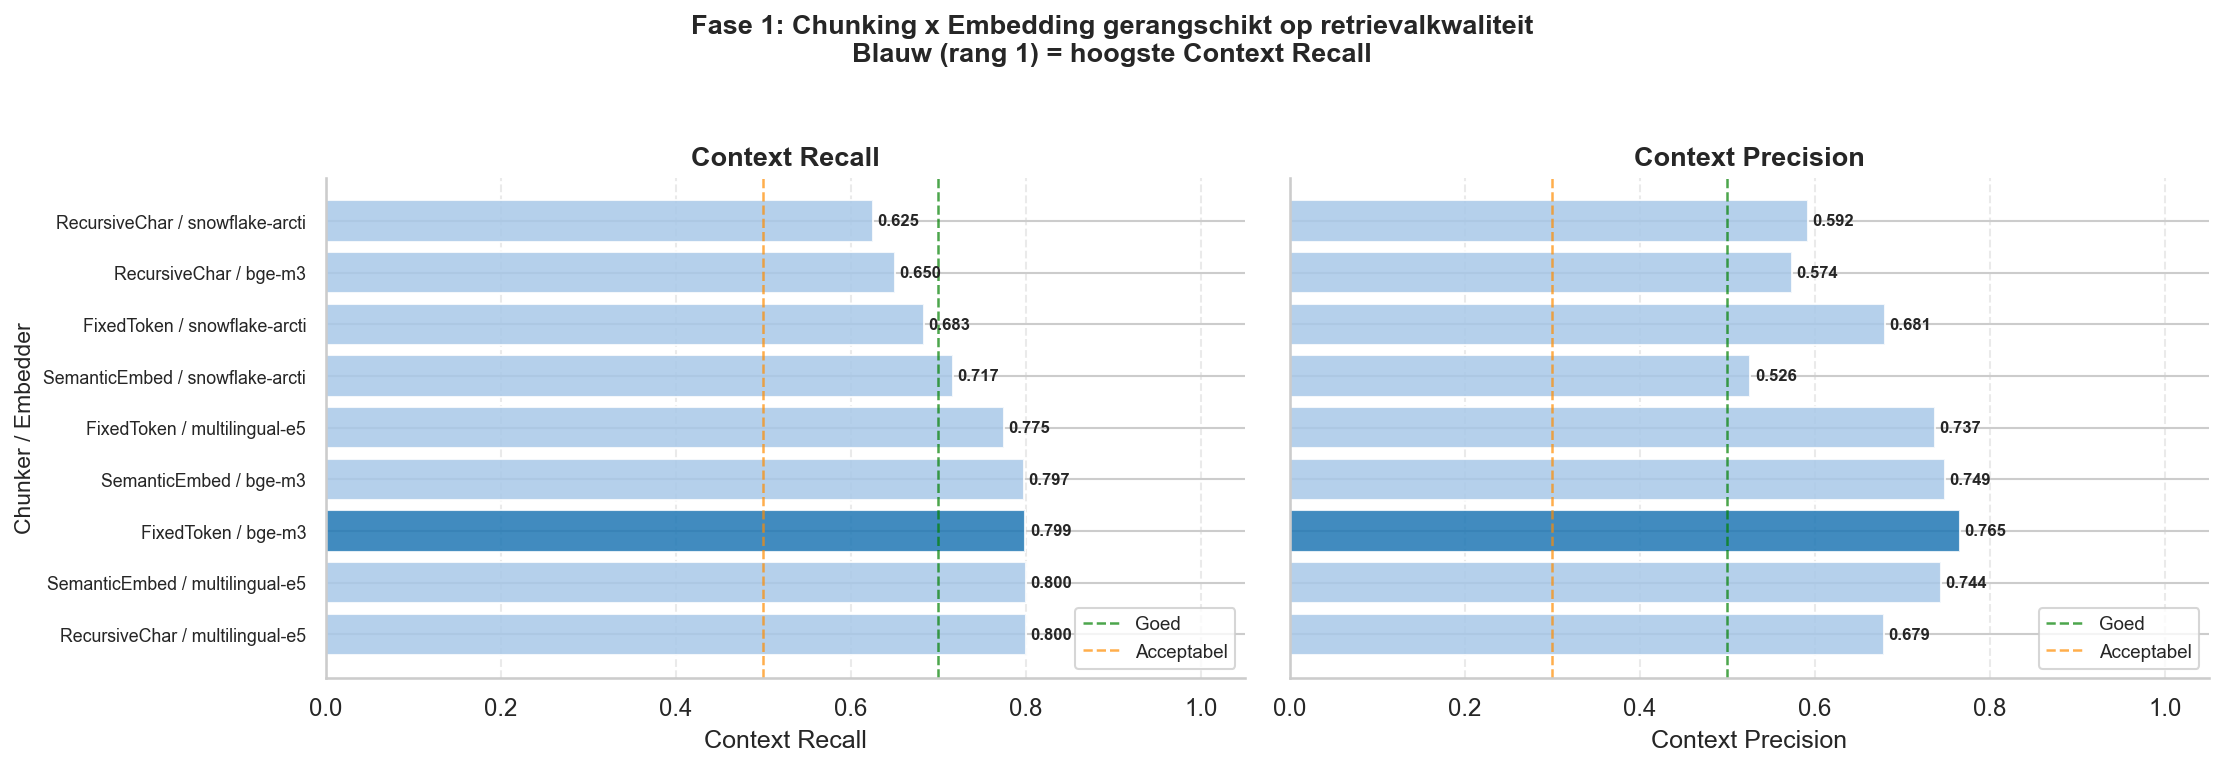
\includegraphics[width=\textwidth]{../graphics/stage1_retriever_ranking.png}
    \caption[Prestatieranking Fase 1: alle Chunker $\times$ Embedder-combinaties]{Prestatieranking van de retrieverfase over alle unieke Chunker $\times$ Embedder-combinaties, gerangschikt op gecombineerde retrievalkwaliteit (Context Recall én Context Precision; blauwe balk = rang~1). \texttt{FixedToken+bge-m3} behaalt rang~1 met $\mu_{\text{CR}} = 0{,}799$ en de hoogste Context Precision van alle combinaties ($\mu_{\text{CP}} = 0{,}765$). \texttt{RecursiveChar+bge-m3} en \texttt{RecursiveChar+Snowflake} bezetten de twee laagste posities, wat het sterk embedder-afhankelijke karakter van de \texttt{RecursiveCharacterSplitter} illustreert.}
    \label{fig:retriever-ranking}
\end{figure}

De combinatie \texttt{FixedToken+bge-m3} behaalt rang~1 met $\mu_{\text{CR}} = 0{,}799$ en de hoogste Context Precision van alle combinaties ($\mu_{\text{CP}} = 0{,}765$). De vaste tokengrens van de \texttt{FixedSizeTokenSplitter} produceert homogene, compact afgebakende chunks die zowel de dense-vector- als de sparse-lexicale retrieval van \texttt{bge-m3} maximaal benutten — een complementariteitseffect dat de simultaan hoge scores op beide retrievalmetrics verklaart. \texttt{RecursiveChar+E5-large} ($\mu_{\text{CR}} = 0{,}800$) en \texttt{SemanticEmbed+E5-large} ($\mu_{\text{CR}} = 0{,}800$) bereiken een marginaal hogere recall maar scoren aanzienlijk lager op precisie ($\mu_{\text{CP}} = 0{,}679$ resp.\ $0{,}744$). De \texttt{RecursiveCharacterSplitter} blijft sterk embedder-afhankelijk: \texttt{Recursive+bge-m3} ($\mu_{\text{CR}} = 0{,}650$) en \texttt{Recursive+Snowflake} ($\mu_{\text{CR}} = 0{,}625$) bezetten de twee laagste posities. Dit bevestigt dat de grotere chunkomvang van de \texttt{RecursiveCharacterSplitter} een kwalitatief sterk embeddingmodel vereist: zonder \texttt{E5-large} tast de semantische diversiteit van de grote chunks de retrieval-nauwkeurigheid aan.

De significante impact van de chunker op \textit{Context Precision} ($H = 6{,}98$, $p = 0{,}031$) wordt structureel zichtbaar in Figuur~\ref{fig:embedder-chunker-precision}. In tegenstelling tot wat de marginale gemiddelden uit Sectie~\ref{subsec:chunker-context-precision} suggereren, onthult het interactie-effect een genuanceerder patroon. De \texttt{FixedSizeTokenSplitter} presteert het meest consistent over alle drie de embeddingmodellen. De \texttt{SemanticEmbeddingChunker} presteert opvallend sterk bij de twee superieure embeddingmodellen (\texttt{bge-m3}: $\mu = 0{,}749$; \texttt{E5-large}: $\mu = 0{,}744$), en evenaart of overstijgt hier de \texttt{FixedSizeTokenSplitter}. De \texttt{RecursiveCharacterSplitter} is consequent het zwakst bij de krachtige embeddingmodellen (\texttt{bge-m3}: $\mu = 0{,}574$; \texttt{E5-large}: $\mu = 0{,}679$). Het scherpste interactie-effect — de causale kern van de kruisende lijnen in de figuur — treedt op bij de combinatie \texttt{Snowflake} $\times$ \texttt{Semantic}: de \texttt{SemanticEmbeddingChunker} zakt bij dit zwakkere embeddingmodel tot $\mu = 0{,}526$. De verklaring voor dit patroon is complementariteit: wanneer een krachtige embedder de semantisch samengestelde chunks nauwkeurig in de vectorruimte representeert, versterken semantisch coherente segmenten de retrieval-precisie. Bij het structureel zwakkere \texttt{Snowflake}-model verdwijnt deze synergie, en worden grotere, semantisch samengestelde chunks een bron van ruis.

\begin{figure}[!htb]
    \centering
    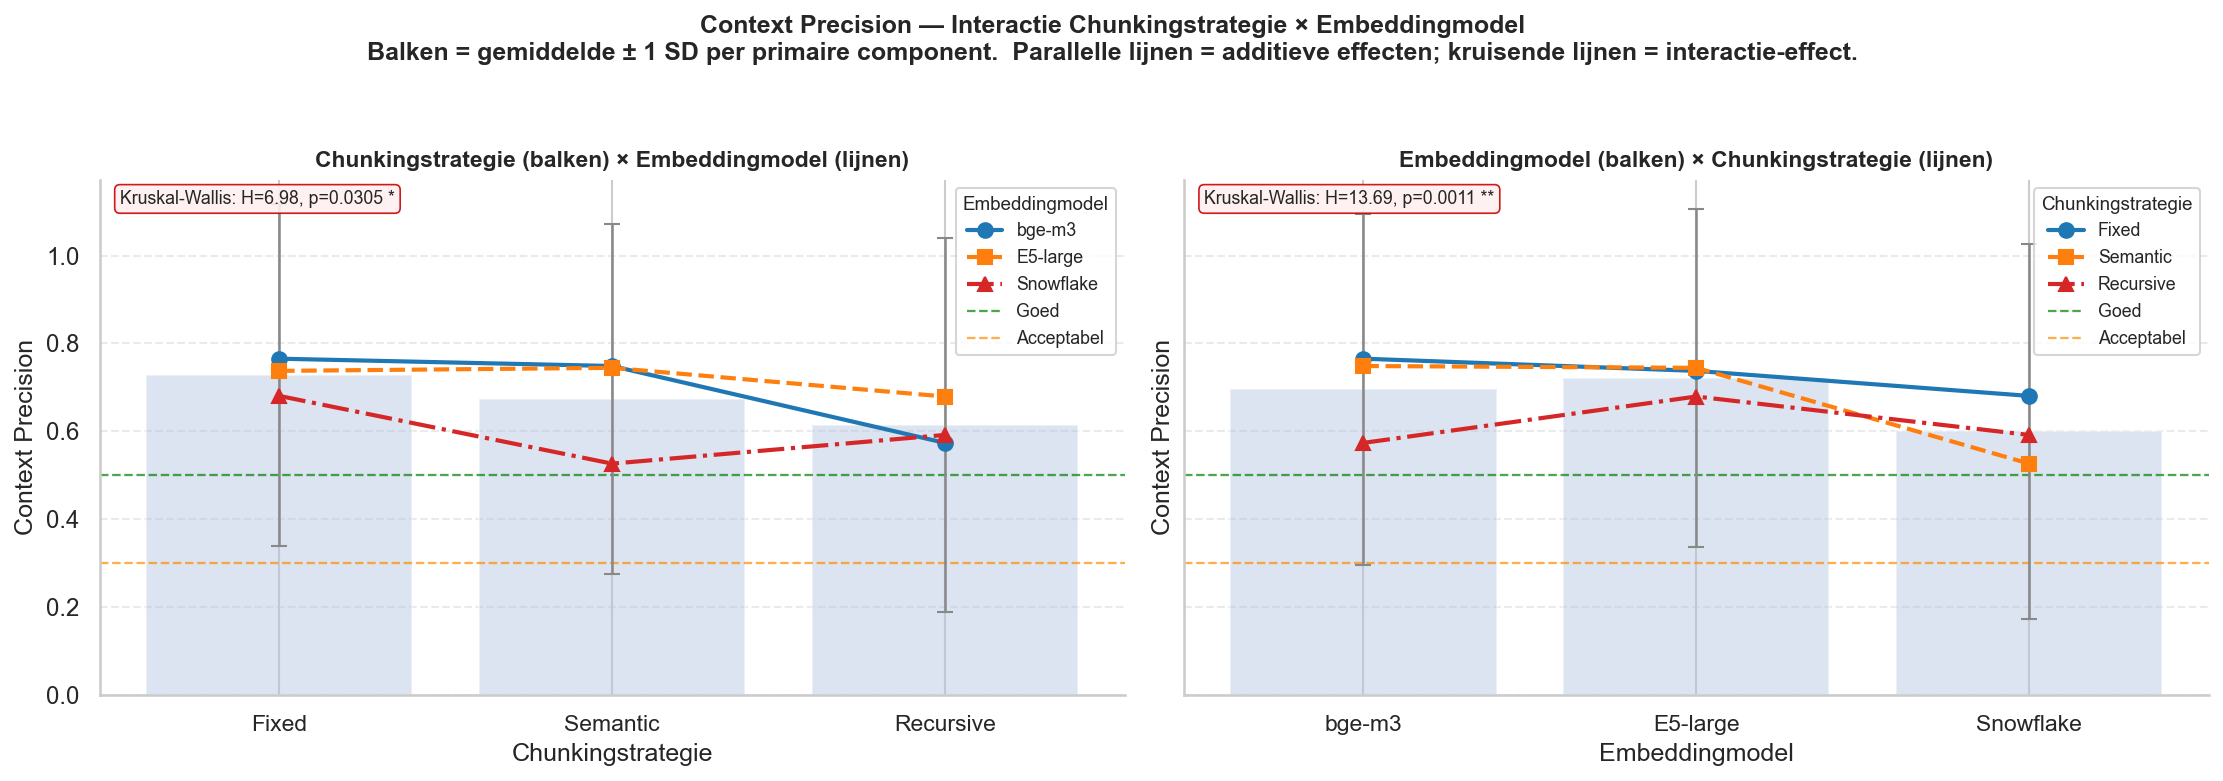
\includegraphics[width=\textwidth]{../graphics/interaction_context_precision_chunker_embedder.png}
    \caption[Interactie-effect chunking $\times$ embedding op Context Precision]{Interactie-effect tussen de chunkingstrategieën en embeddingmodellen op de Context Precision-metriek. De \texttt{FixedSizeTokenSplitter} is het meest consistent. De \texttt{SemanticEmbeddingChunker} presteert sterk bij \texttt{bge-m3} ($\mu = 0{,}749$) en \texttt{E5-large} ($\mu = 0{,}744$) maar zakt scherp bij \texttt{Snowflake} ($\mu = 0{,}526$). De \texttt{RecursiveCharacterSplitter} blijft consequent het zwakst bij de krachtige embeddingmodellen.}
    \label{fig:embedder-chunker-precision}
\end{figure}

\section{Globale resultatenvergelijking}
\label{sec:globale-vergelijking}

De benchmark-resultaten van alle 27 geteste \gls{rag}-pipelineconfiguraties worden in deze sectie globaal geanalyseerd en vertaald naar een beslissingsboom die toekomstige implementatoren begeleidt bij de configuratiekeuze op basis van concrete metriekdrempels.

\subsection{Globale analysepatronen}
\label{subsec:globale-analysepatronen}

De kwantitatieve vergelijking van de benchmark-resultaten brengt drie fundamentele patronen naar voren die de configuratieselectie structureren.

\paragraph{Dominantie van Source Attribution als differentiërende factor}

De combinatie \texttt{RecursiveCharacterSplitter | multilingual-e5-large-instruct | Gemma-3-27b-it} is als enige configuratie in staat om tegelijkertijd aan alle drie kritische drempelwaarden te voldoen: de \texttt{RecursiveCharacterSplitter} is de enige chunkingstrategie die SA\,$\geq$\,40\,\% haalt (46{,}7\,\%; Sectie~\ref{subsec:chunker-source-attribution}), \texttt{E5-large} levert de hoogste Context Recall ($\mu = 0{,}792$; Sectie~\ref{subsec:embedding-prestaties}) en \texttt{Gemma} behaalt de numeriek sterkste F\,+\,SA-combinatie van alle LLM's (Sectie~\ref{subsec:llm-prestaties}). Het strategische voordeel ligt niet in de beste gemiddelde retrievalkwaliteit — de \texttt{RecursiveCharacterSplitter} is sterk embedder-afhankelijk en scoort zwak met \texttt{bge-m3} en \texttt{Snowflake} (Sectie~\ref{sec:meervoudige-interactie}) — maar in de unieke bronvermeldingssuperioriteit die geen andere componentcombinatie kan evenaren.

\textit{Source Attribution} is de meest differentiërende metric: in een \gls{csrd}-compliancecontext is de juridische traceerbaarheid van een claim minstens even belangrijk als de inhoudelijke volledigheid. Configuraties die bronnen correct citeren combineren deze traceerbaarheid structureel met een sterke contextdekking.

\paragraph{E5-large als meest veelzijdig embeddingmodel}

Een kenmerkende observatie is dat het \texttt{multilingual-e5-large-instruct}-model het meest veelzijdig presteert over de vijf kwaliteitsmetrics. Het combineert de beste \textit{Context Recall} ($\mu = 0{,}792$; Sectie~\ref{subsec:embedding-prestaties}), is statistisch equivalent aan \texttt{bge-m3} voor \textit{Context Precision} ($p_{\text{holm}} = 0{,}192$), en vertoont geen meetbare penalisering op \textit{Source Attribution}. Configuraties die steunen op \texttt{Snowflake} vertonen — ongeacht chunker of LLM — op de primaire retrieval- en relevantie-metrics (CR, CP en AR) de zwakste absolute prestaties. De lagere retrievalkwaliteit werkt als een cascade stroomafwaarts door: onvolledige context leidt tot slechtere faithfulness, meer weigeringen bij \texttt{Mistral} en lagere SA-scores voor het gehele pijplijnsegment.

\paragraph{LLM-keuze: geen statistisch onderscheid op kwaliteitsmetrics}

Omdat geen enkel LLM statistisch significant beter presteert op \textit{Faithfulness} of \textit{Answer Relevancy}, wordt de LLM-keuze in dit experiment niet primair op kwaliteitsgronden beslist. \texttt{Gemma-3-27b-it} behaalt de hoogste gemiddelde faithfulness ($\mu = 0{,}657$, niet significant) en het hoogste SA-gemiddelde ($\mu = 0{,}344$), en is daarmee op Faithfulness en Source Attribution de numeriek sterkste keuze wanneer de statistisch niet-significante LLM-effecten als richtinggevend worden geïnterpreteerd. \texttt{Llama-3.3-70B-Instruct} presteert numeriek het zwakst op faithfulness ($\mu = 0{,}583$) en source attribution ($\mu = 0{,}328$). \texttt{Mistral-Small-2603} scoort numeriek het laagst op SA ($\mu = 0{,}278$), deels als gevolg van de weigeringsparadox beschreven in Sectie~\ref{subsec:mistral-paradox}, waarbij correcte weigeringen bij gebrekkige context de SA-score structureel drukken.

\subsection{Beslissingsboom voor RAG-configuratieselectie}
\label{subsec:beslisboom}

Op basis van de experimentele resultaten is een beslissingsboom opgesteld die via drie concrete metriekdrempels naar de optimale \gls{rag}-pipelineconfiguratie leidt. De drie criteria zijn: \textbf{Source Attribution} (SA\,$\geq$\,40\,\%; traceerbaarheid naar brondocumentpagina's), \textbf{Answer Relevancy} (AR\,$\geq$\,0{,}65; gefocuste, on-topic antwoorden) en \textbf{Faithfulness} (F\,$\geq$\,0{,}65; hallucinatiepreventie). Door de boom van boven naar beneden te doorlopen en bij elke knoop \textbf{JA} of \textbf{NEE} te kiezen op basis van de eigen inzetcontext, wordt exact de configuratie bereikt die aan die eisen voldoet.

Het \gls{llm} is in alle paden \texttt{Gemma-3-27b-it}: geen enkel model vertoont een statistisch significant effect op faithfulness of answer relevancy ($H{=}5{,}78$, $p{=}0{,}056$), maar \texttt{Gemma} scoort numeriek het best op Faithfulness ($\mu{=}0{,}657$). \texttt{Mistral} behaalt numeriek de hoogste Answer Relevancy ($\mu{=}0{,}676$) maar wordt vermeden wegens de SA-weigeringsparadox (Sectie~\ref{subsec:mistral-paradox}); \texttt{Llama} wegens de laagste faithfulness-trend ($\mu{=}0{,}583$). \texttt{Snowflake Arctic Embed} is voor alle paden uitgesloten wegens de zwakste retrieval-kwaliteit op CR, CP en AR (Sectie~\ref{subsec:embedding-prestaties}).

\begin{figure}[p]
  \centering
  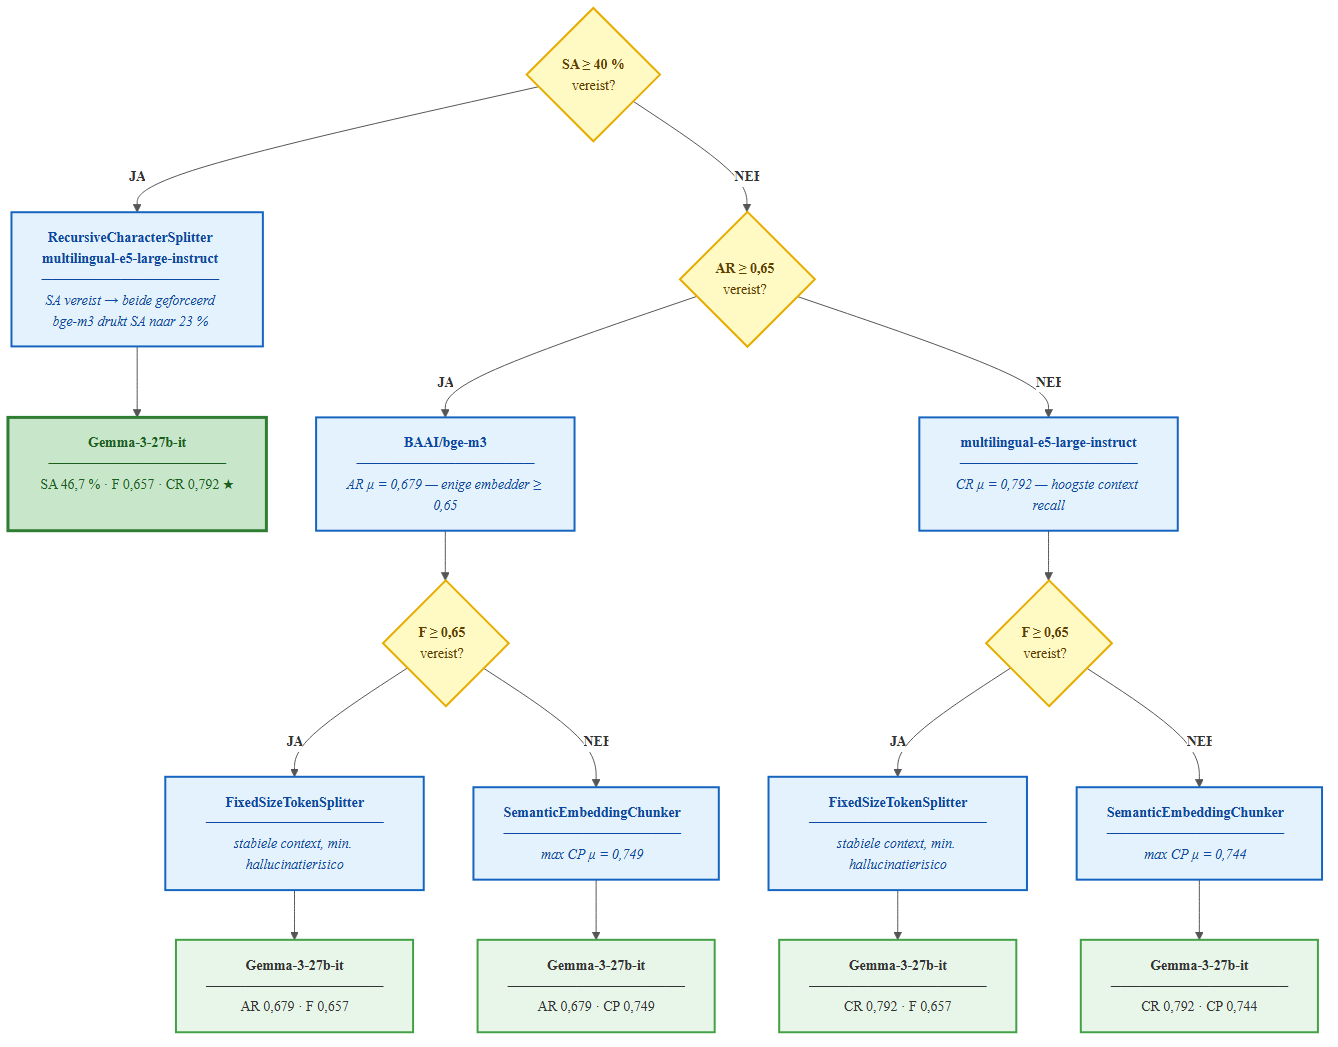
\includegraphics[width=\textwidth]{../graphics/beslisboom}
  \caption[Beslissingsboom voor RAG-configuratieselectie op basis van drie metriekdrempels]{Beslissingsboom voor de selectie van de optimale \gls{rag}-pipelineconfiguratie. De drie drempelvragen zijn SA\,$\geq$\,40\,\% (Knoop~1), AR\,$\geq$\,0{,}65 (Knoop~2) en F\,$\geq$\,0{,}65 (Knoop~3). Beantwoord elke knoop JA of NEE naargelang de minimumeis van uw inzetcontext. Het \gls{llm} is in alle paden \texttt{Gemma-3-27b-it}. SA\,$\geq$\,40\,\% is uitsluitend haalbaar met \texttt{RecursiveCharacterSplitter}\,+\,\texttt{E5-large}; AR\,$\geq$\,0{,}65 uitsluitend met \texttt{bge-m3}; SA en AR zijn structureel incompatibel. De $\bigstar$-configuratie is de globale winnaar op alle drie de drempelcriteria (Sectie~\ref{subsec:globale-analysepatronen}).}
  \label{fig:beslisboom}
\end{figure}

\subsubsection{Toelichting bij de drempelkeuzes}
\label{subsec:beslisboom-toelichting}

De drie drempelkeuzes in de boom zijn geselecteerd op basis van de statistisch meest significante componenteffecten en de kritische succesfactoren van de inzetcontext. Hieronder wordt per knoop de empirische onderbouwing van de drempel toegelicht.

\paragraph{Knoop 1 — SA $\geq$ 40\,\% vereist?}
Source Attribution is de meest onderscheidende metric voor de chunker-keuze en de enige waarvoor een statistisch significante componentafhankelijkheid bestaat. \texttt{RecursiveCharacterSplitter} is de \emph{enige} strategie die SA\,$\geq$\,40\,\% haalt: 46{,}7\,\% correct (84/180 configuratieruns), significant beter dan \texttt{Fixed} (23{,}3\,\%) en \texttt{Semantic} (25{,}0\,\%), $p_{\text{holm}}{<}0{,}001$ (Sectie~\ref{subsec:chunker-source-attribution}). De grotere chunkgrenzen van de recursieve splitter bewaren de positie van de \texttt{<<<PAGE~X>>>}-markeerders intakt, waardoor de \texttt{ChunkMetaCleaner} paginanummers correct kan koppelen. Op het JA-pad is ook de embedder-keuze geforceerd: \texttt{E5-large} vermijdt de SA-penalty die \texttt{bge-m3} treft door zijn hybride RRF-retrieval — bij \texttt{bge-m3} daalt de correcte SA tot slechts 23\,\%, wat elke meerwaarde van Recursive tenietdoet (Sectie~\ref{sec:meervoudige-interactie}).

\paragraph{Knoop 2 — AR $\geq$ 0{,}65 vereist?}
Wanneer SA\,$<$\,40\,\% aanvaardbaar is, splitst de boom op de Answer Relevancy-drempel. \texttt{BAAI/bge-m3} is het \emph{enige} model dat AR\,$\geq$\,0{,}65 haalt: $\mu{=}0{,}679$, significant beter dan \texttt{Snowflake} ($\mu{=}0{,}546$; $p_{\text{holm}}{<}0{,}001$) en numeriek beter dan \texttt{E5-large} ($\mu{=}0{,}635$; $p_{\text{holm}}{=}0{,}129$, niet sig., Sectie~\ref{subsec:embedding-prestaties}). De multi-vector architectuur (dense\,+\,sparse) van \texttt{bge-m3} herkent on-topic passages en vertaalt dit in gefocuste antwoorden. De trade-off is een lagere SA ($\mu{=}0{,}233$) — aanvaardbaar enkel wanneer het NEE-antwoord op Knoop~1 correct is. \texttt{E5-large} is aangewezen wanneer AR\,$<$\,0{,}65 voldoet: het haalt de hoogste Context Recall ($\mu{=}0{,}792$; $p_{\text{holm}}{=}0{,}019$ t.o.v.\ Snowflake) en is statistisch equivalent aan \texttt{bge-m3} voor Context Precision ($p_{\text{holm}}{=}0{,}192$).

\paragraph{Knoop 3 — F $\geq$ 0{,}65 vereist?}
De derde drempel bepaalt de chunker-morfologie vanuit een risicobeheersperspectief. Wanneer faithfulness een harde eis is ($\geq$\,0{,}65), is \texttt{FixedSizeTokenSplitter} de aangewezen keuze: vaste token-grenzen produceren homogene, voorspelbare chunks die het risico op incoherente contextfragmenten minimaliseren. Incoherente context is een van de mechanismen die een \gls{llm} tot hallucinaties kan triggeren, los van de significantie van het \gls{llm}-hoofdeffect. \texttt{Gemma} wordt in dit pad gehandhaafd als generatieve engine wegens zijn numeriek hoogste faithfulness ($\mu{=}0{,}657$). Op het NEE-pad is faithfulness secundair en wordt de chunker-keuze bepaald door Context Precision: \texttt{SemanticEmbeddingChunker} haalt CP\,$\mu{=}0{,}749$ bij \texttt{bge-m3} en CP\,$\mu{=}0{,}744$ bij \texttt{E5-large} (Sectie~\ref{subsec:chunker-context-precision}). Het chunker~$\times$~embedder-interactie-effect ($H{=}6{,}98$, $p{=}0{,}031$) vormt geen risico meer: \texttt{Snowflake} is reeds uitgesloten in alle paden van de boom.

%%----------------------------------------------------------------------
\section{Synthese van de resultaten}
\label{sec:synthese}

De vier analytische lagen van dit hoofdstuk — methodologische validatie, cross-component variantie-analyse, geïsoleerde componentanalyse en interactie-effecten — convergeren naar een coherent en intern consistent beeld van de systeemdynamica. Deze sectie brengt de voornaamste bevindingen samen in een geïntegreerd overzicht.

\paragraph{Componenthiërarchie: embedder \texorpdfstring{$>$}{>} chunker \texorpdfstring{$>$}{>} LLM.}
De meest fundamentele bevinding van dit experiment is de duidelijke en statistisch verdedigbare hiërarchie in componenteffecten. Het \textbf{embeddingmodel} is de dominante kwaliteitshefboom van de pipeline: het is de primaire driver voor context recall ($H = 7{,}54$, $p = 0{,}023$), context precision ($H = 13{,}69$, $p = 0{,}001$) en answer relevancy ($H = 13{,}82$, $p = 0{,}001$), en een significante secundaire driver voor source attribution ($H = 8{,}97$, $p = 0{,}011$). De \textbf{chunkingstrategie} is de primaire driver voor source attribution ($H = 28{,}14$, $p < 0{,}001$) — de metriek die in een \gls{csrd}-compliancecontext juridisch het meest cruciaal is — en vertoont een statistisch significante interactie met het embeddingmodel op context precision. Het \textbf{\gls{llm}} vertoont op geen enkele van de vijf metrics een statistisch significant hoofdeffect. Deze hiërarchie impliceert dat optimalisatie-inspanningen het meest rendabel zijn wanneer ze gericht zijn op de upstream vectorisatie- en chunkfase, en niet op de selectie van een krachtigere generatieve engine.

\paragraph{Winnende configuratie en haar strategisch voordeel.}
De combinatie \texttt{RecursiveCharacterSplitter + multilingual-e5-large-instruct + Gemma-3-27b-it} is als enige van de 27 configuraties in staat om tegelijkertijd aan alle drie de kritische drempelwaarden te voldoen: SA\,$\geq$\,40\,\% (46{,}7\,\%), CR\,$\geq$\,0{,}75 ($\mu = 0{,}792$) en F\,$\geq$\,0{,}65 ($\mu = 0{,}657$). Haar strategische voordeel ligt niet in de beste absolute retrievalkwaliteit — de \texttt{RecursiveCharacterSplitter} is sterk embedder-afhankelijk en presteert zwak met \texttt{bge-m3} of \texttt{Snowflake} (Sectie~\ref{sec:meervoudige-interactie}) — maar in de unieke combinatie van de enige chunkingstrategie die SA\,$\geq$\,40\,\% haalt met het embeddingmodel dat die SA-drempel niet tenietdoet.

\paragraph{Verrassende bevinding: \texttt{E5-large} trotseerd zijn eigen architectuurbeperking.}
Ondanks een maximale inputlengte van 512 tokens — waardoor ruwweg 35\,\% van de chunk-inhoud structureel afgekapt wordt — behaalt \texttt{multilingual-e5-large-instruct} de hoogste context recall van alle drie embeddingmodellen. De verklaring ligt in drie samenlopende mechanismen: de domeingerichte instruction-tuning compenseert de beperkte contextcapaciteit, \gls{esg}-compliancedocumenten zijn structureel \textit{front-loaded} waardoor het retrieval-relevante signaal vrijwel altijd binnen de eerste 512 tokens valt, en langere embeddings zijn vatbaarder voor het \textit{verdunnings-effect} waarbij irrelevante perifere tokens het semantische signaal verzwakken. Dit resultaat nuanceert de intuïtieve aanname dat een groter contextvenster altijd leidt tot betere retrieval.

\paragraph{Structurele SA/AR-incompatibiliteit.}
De data onthult een fundamentele spanningsverhouding tussen source attribution en answer relevancy die niet via hyperparameterafstemming kan worden opgeheven. Het enige embeddingmodel dat AR\,$\geq$\,0{,}65 haalt (\texttt{bge-m3}, $\mu = 0{,}679$) vertoont tegelijk de laagste SA ($\mu = 0{,}233$). Omgekeerd vereist SA\,$\geq$\,40\,\% \texttt{E5-large} als embedder, wat AR beperkt tot $\mu = 0{,}635$. Deze trade-off is een structurele eigenschap van de hybride RRF-retrieval van \texttt{bge-m3}: de sparse lexicale gewichten selecteren bij voorkeur tabelrijen met \gls{esg}-termen die hoog in de ranking belanden maar centraal op een pagina staan — buiten het bereik van de \texttt{<<<PAGE~X>>>}-markeerders. SA en AR zijn daarmee in de huidige pipelineopzet structureel incompatibel; een implementator moet expliciet kiezen welke van de twee prioriteit heeft.

\paragraph{De Snowflake-cascade en de Mistral-weigeringsparadox.}
Twee systeeminteracties illustreren hoe een zwakke upstream component disproportionele downstream-effecten induceert. De zwakke retrievalkwaliteit van \texttt{Snowflake Arctic Embed} — ondanks zijn hoge \gls{clef}-benchmarkscore voor Italiaanse retrieval — zorgt voor een cascade die de faithfulness, context precision en source attribution van de volledige \texttt{Snowflake}-configuraties aantast. Dit cascade-effect wordt versterkt wanneer \texttt{Snowflake} gekoppeld is aan \texttt{Mistral-Small}: de Mistral-weigeringsparadox zorgt ervoor dat correcte weigeringen bij onvolledige context geregistreerd worden als SA-score nul, waardoor de \texttt{Snowflake-Mistral}-combinaties disproportioneel slecht scoren. Beide patronen bevestigen dat de LLM pas optimaal kan functioneren wanneer de upstream retrievalfase kwalitatief hoogwaardig is.

\paragraph{Betrouwbaarheid van de evaluatiemetrics.}
De menselijke validatiestudie (Sectie~\ref{sec:methodologische-validatie}) toont een sterk gedifferentieerd betrouwbaarheidslandschap. \textit{Context Recall} is de robuuste ankermetriek van dit onderzoek ($\rho = 0{,}973$): vergelijkingen op basis van CR zijn direct interpreteerbaar. \textit{Context Precision} en \textit{Source Attribution} zijn matig betrouwbaar ($\rho \approx 0{,}36$--$0{,}58$) en vertonen een systematische positieve bias, wat betekent dat de geautomatiseerde scores de werkelijke kwaliteit overschatten. \textit{Faithfulness} en \textit{Answer Relevancy} zijn de minst betrouwbare metrics ($\rho = 0{,}257$ resp.\ $0{,}460$), mede door de taalkundige complexiteit van Italiaanse technisch-juridische terminologie die de strikte claim-verificatie van \gls{ragas} bemoeilijkt. Rangvergelijkingen tussen configuraties zijn op al deze metrics betrouwbaarder dan absolute drempeloordelen.